\documentclass[aspectratio=169,xcolor=dvipsnames]{beamer}
\usetheme{SimplePlus}

% Math
\usepackage{nicefrac}

% Tipography stuff
\usepackage{booktabs} % Allows the use of \toprule, \midrule and \bottomrule in tables
\usepackage[english]{babel}
\usepackage{csquotes}
\usepackage{microtype}
\usepackage{pdfpages}
\usepackage{fontawesome5}
\usepackage{soul}
\usepackage{euler}
\usepackage{algorithm2e}
\usepackage{animate}
\usepackage{ifthen}
\usepackage{multirow}
\usepackage{multicol}
\usepackage{pgfplotstable}

% Bibliography
\usepackage[giveninits,style=authoryear-comp,backend=biber]{biblatex}
\addbibresource{../fracbiblio.bib}
\newcommand\unnumbered{\setbeamertemplate{footline}{}}%\addtocounter{framenumber}{-1}
\renewcommand*{\bibfont}{\normalfont\small}

% Figures
\usepackage{tikz,pgfplots}
\usetikzlibrary{calc,arrows,patterns,matrix,external}
\usepackage{subfig}
\usepackage{graphicx} % Allows including images
\usepackage[american]{circuitikz}
\usepackage{tikz-network}
\tikzexternalize[prefix=Figures/] % activate and define figures/ as cache folder
\usepackage{mathtools}

% Links
\usepackage{hyperref}
\hypersetup{colorlinks,linkcolor=,urlcolor=MidnightBlue}

% Code
\usepackage{minted}

% Block matrices
\newcommand{\bigzero}{\mbox{\normalfont\Large\bfseries 0}}
\newcommand{\rvline}{\hspace*{-\arraycolsep}\vline\hspace*{-\arraycolsep}}
\newcommand{\R}{\mathbb{R}}
\newcommand{\bone}{{\bf 1}}
\newcommand{\evec}{{\bf e}}
\newcommand{\dvec}{{\bf d}}
\newcommand{\xvec}{{\bf x}}
\newcommand{\yvec}{{\bf y}}
\newcommand{\qvec}{{\bf q}}
\newcommand{\svec}{{\bf s}}
\newcommand{\pvec}{{\bf p}}
\newcommand{\tvec}{{\bf t}}
\definecolor{Ao}{rgb}{0.0, 0.5, 0.0}
\setlength{\tabcolsep}{0.3em}


\author{Fabio Durastante}
\title{An introduction to fractional calculus}
\subtitle{Fundamental ideas and numerics}
\institute{Università di Pisa\\\href{mailto:fabio.durastante@unipi.it}{\faEnvelope\;fabio.durastante@unipi.it}\\\href{https://fdurastante.github.io}{\faFirefox\;fdurastante.github.io}}
\date{October, 2022}

\newcommand{\de}{{\rm d}}


\begin{document}
	
	{\unnumbered
		\begin{frame}[t,plain,noframenumbering]
			\titlepage
			\vspace{-4em}
\includegraphics[width=2cm]{frame.png}
		\end{frame}
	}

	\section{Sylvester with quasiseparable matrices}
	
	\begin{frame}{Sylvester with quasiseparable matrices}
	Let's start again from the problem we wanted to solve
	\[
	A X + X B^T = C, \qquad A \in \mathbb{R}^{n \times n}, \;\; B \in \mathbb{R}^{m \times m}, \;\; X,C \in \mathbb{R}^{n \times m},
	\]
	with $A$, $B$, and $C$ \textbf{quasiseparable}
	\begin{columns}
		\begin{column}{0.45\columnwidth}
		\begin{block}{Quasiseparable matrix}
			A matrix $A$ is \emph{quasiseparable} of order $k$ if the maximum of the ranks of all its submatrices contained in the strictly upper or lower part is less or equal than~$k$. 
		\end{block}
	\end{column}
	\begin{column}{0.45\columnwidth}
	\centering
	\definecolor{lowrankcolor}{rgb}{.75,.75,.75}
	\begin{tikzpicture}[scale=1.2]
		\draw [thick] (0,0) rectangle (2,2);
		\draw (0,2) -- (2,0);
		
		% Low rank blocks
		\fill [lowrankcolor] (0.05,1.25) rectangle (0.65,.05);
		\fill [lowrankcolor] (0.8,1.4) rectangle (1.75,1.75);
		
		% ... and their representation as outer products
		\fill [lowrankcolor] (-1.8,1.25) rectangle (-1.65,.05);
		\fill [lowrankcolor] (-1.6,1.25) rectangle (-1.1,1.1);
		\draw[->] (-1.55,0.6) -- (-.05,0.6);
		
		\fill [lowrankcolor] (2.5,1.75) rectangle (2.65,1.4);
		\fill [lowrankcolor] (2.7,1.75) rectangle (3.2, 1.6);
		\draw [<-] (1.8,1.575) -- (2.45,1.575);
	\end{tikzpicture}
	\end{column}
	\end{columns}
	\[	\text{\textcolor{Goldenrod}{\faLightbulb}}\; \text{We have seen that $A$, $B$, and $C$ quasiseparable } \Rightarrow\,\begin{array}{c} X\; \text{with \alert{decay of the singular values}}\\\text{of off-diagonal blocks of }C.\end{array}
	\]
	\end{frame}

	\begin{frame}{Sylvester with quasiseparable matrices}
		
	\begin{alertblock}{Theorem~\parencite[Theorem~2.12]{MR3867617}}
		Let $A, B$ be matrices of quasiseparable
		rank $k_A$ and $k_B$ respectively and such that $W(A) \subseteq E$ and 
		$W(-B) \subseteq F$. Consider 
		the Sylvester equation $AX + XB = C$, with $C$ of
		quasiseparable rank $k_C$. Then a generic off-diagonal block $Y$ of
		the solution $X$ satisfies
		\[
		\frac{\sigma_{1 + k\ell}(Y)}{\sigma_1(Y)} \leq \mathcal C^2\cdot Z_{\ell}(E, F), \qquad k:=k_A+k_B+k_C. 
		\]
		Where $Z_{\ell}(E, F)$ is the solution of the \textbf{Zolotarev problem} 
		\[Z_\ell(E, F) \triangleq \inf_{r(x) \in \mathcal R_{\ell,\ell}}
		\frac{\max_{x \in E} |r(x)|}{\min_{y \in F} |r(y)|}, \qquad
		\ell \geq 1, 
		\]
		for $\mathcal R_{\ell,\ell}$ is the set of rational functions of degree
		at most $(\ell,\ell)$, and $\mathcal{C}$ is the Crouzeix universal constant.
	\end{alertblock}
		
	\end{frame}

	\begin{frame}{Sylvester with quasiseparable matrices}
		
	\faQuestionCircle\; Do the \emph{decaying singular values} in the blocks implies the existence of a \textbf{quasiseparable approximant}?
	
	\begin{block}<2->{$\epsilon$-quasiseparable matrices of rank $k$ ($\varepsilon$-qsrank $k$)}
		We say that $A$ has \alert{\emph{$\epsilon$-quasiseparable rank $k$}} if, for
	every off-diagonal block $Y$, $\sigma_{k+1}(Y) \leq \epsilon$. If the
	property holds for the lower (respectively upper) offdiagonal blocks,
	we say that $A$ has lower (respectively upper) $\epsilon$-quasiseparable rank $k$. 
	\end{block}

	\begin{columns}
	\begin{column}{0.45\columnwidth}
	\only<3-4>{\begin{exampleblock}<3->{\small\faEye\,Submatrices and off-diagonal blocks}\small
	If a matrix $A$ has $\epsilon$-quasiseparable rank $k$,
	then any of its principal submatrix $A'$ has $\epsilon$-quasiseparable rank $k$.\\[1em]
	
	Any off-diagonal block $Y$ of $A'$ is also an off-diagonal
	block of $A$ $\Rightarrow$ $\sigma_{k+1}(Y) \leq \epsilon$. 
	\end{exampleblock}}
	\begin{onlyenv}<5->
		
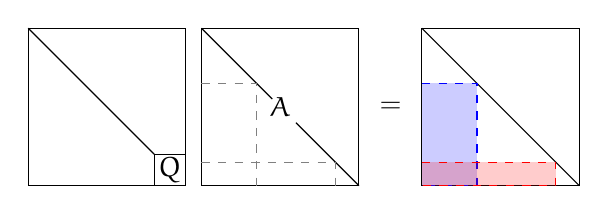
\begin{tikzpicture}
	% Q 
	\draw (0,0) rectangle (2,2);
	\draw (0,2) -- (1.6,0.4);
	\draw (1.6,0) rectangle (2,0.4);
	\node at (1.8,0.2) { $Q$ };
	
	% A
	\draw (2.2,0) rectangle (4.2,2);
	\draw (2.2,2) -- (3.1,1.1); \draw (3.4,0.8) -- (4.2,0);    
	\node at (3.2,1) { $A$ };
	
	% Off-diagonal blocks
	\draw[dashed,gray] (2.2,1.3) -- (2.9,1.3) -- (2.9,0);
	\draw[dashed,gray] (2.2,0.3) -- (3.9,0.3) -- (3.9,0);    
	
	\node at (4.6,1) { $=$ };
	
	% QA
	\draw (5,0) rectangle (7,2);
	\draw (5,2) -- (7,0);
	
	% Off-diagonal blocks
	\draw[dashed,blue,fill,fill opacity=0.2] (5,1.3) -- (5.7,1.3) -- (5.7,0) -- (5,0);
	\draw[dashed,red,fill,fill opacity=0.2] (5,0.3) -- (6.7,0.3) -- (6.7,0) -- (5,0);
\end{tikzpicture}
	\end{onlyenv}
	\end{column}
	\begin{column}{0.45\columnwidth}
	\only<4>{For $\oplus$ the direct sum
		
	\begin{alertblock}<4->{Technical lemma}
	Let $A$ be a matrix with $\epsilon$-quasiseparable rank $k$,
	$Q$ any $(k+1) \times (k+1)$
	unitary matrix. Then, $(I_{n-k-1} \oplus Q) A$ also has
	$\epsilon$-quasiseparable rank $k$. 
	\end{alertblock}}

	\only<5>{\centering $Q$ acts on the \textcolor{blue}{tall block of $A$} without changing its singular values, while \alert{the small one} has small
		rank thanks to the small number of rows.}

	\end{column}
	\end{columns}
		
	\end{frame}

	\begin{frame}{Sylvester with quasiseparable matrices}
		
	\begin{alertblock}{Theorem \parencite[Theorem 2.16]{MR3867617}}
	Let $A$ be of $\epsilon$-quasiseparable rank $k$, for $\epsilon > 0$.
	Then, there exists a matrix $\delta A$ of norm
	bounded by $\|\delta A\|_2 \leq 2 \sqrt{n} \cdot \epsilon$
	so that $A + \delta A$ is $k$-quasiseparable. 
	\end{alertblock}

	\begin{columns}
	\begin{column}{0.5\columnwidth}
	\vspace{1em}	
	
	\onslide<2->{\begin{quote}
		\faEye\; A matrix with $\epsilon$-quasiseparable
		rank of $k$ can be \alert{well-approximated} by a matrix with exact
		quasiseparable rank $k$!
	\end{quote}}
	\vspace{2em}

	\onslide<3->{\begin{quote}
	\faEye\; If the \textbf{spectra} of $A$ and $-B$ are \textbf{well-separated} in the Zolotarev sense, we can \textbf{preserve structure}!
	\end{quote}}
	\end{column}
	\begin{column}{0.5\columnwidth}
	\centering
	
	\onslide<4->{\faQuestionCircle\; How can we operate efficiently with these matrix structures?}
	
	\begin{itemize}
		\item[\faMoneyBill]<5-> \textbf{Reduced cost} for BLAS-like operations, 
		\item[\faMemory]<6-> \emph{Contained storage cost}.
		\item[\textcolor{Goldenrod}{\faLightbulb}]<7-> Hierarchical matrix formats! 
	\end{itemize}
	
	\end{column}
	\end{columns}
	
	\end{frame}

	\subsection{HODLR-matrices}
	
	\begin{frame}{Hierarchical matrix formats}
	
	There exist \textbf{many hierarchical matrix formats}:
	\begin{columns}
	\begin{column}{0.6\columnwidth}
	\begin{itemize}
	\item[\faWrench] $\mathcal{H}$-Matrices,  
	\item[\faWrench] $\mathcal{H}^2$-Matrices, 
	\item[\only<1,2>{\faWrench}\only<3->{\faHammer}] \alert<3>{\textbf{H}ierarchical \textbf{O}ff-\textbf{D}iagonal \textbf{L}ow-\textbf{R}ank (HODLR)},  
	\item[\faWrench] \textbf{H}ierarchically \textbf{S}emi\textbf{S}eparable (HSS),
	\item[\faWrench] \textbf{B}lock \textbf{L}ow-\textbf{R}ank (BLR).
	\end{itemize}
	\end{column}
	\begin{column}{0.4\columnwidth}
	\centering
	\only<4->{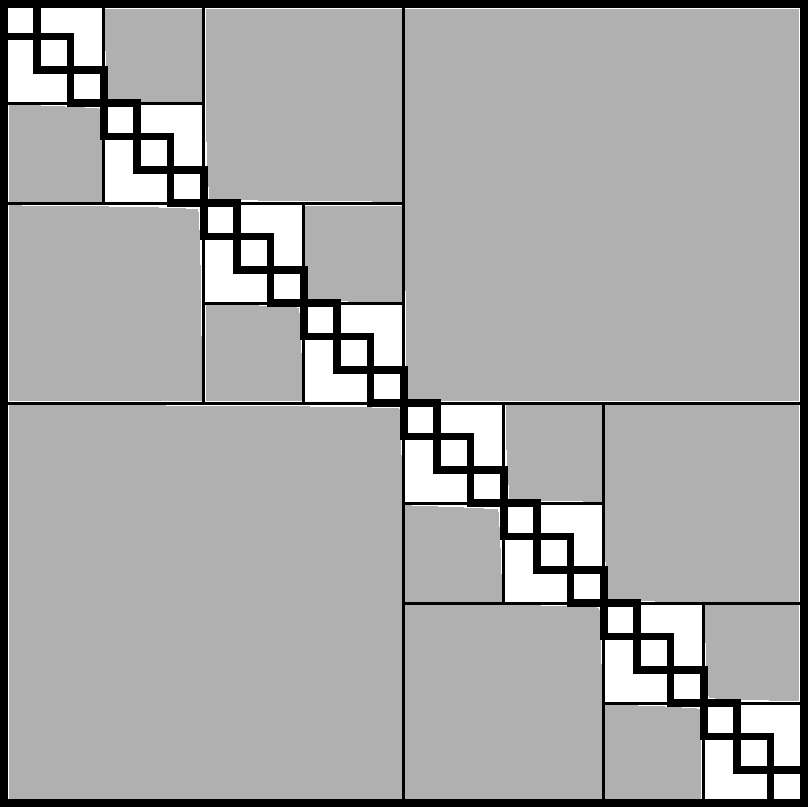
\includegraphics[width=0.7\columnwidth]{figura4.pdf}}
	\end{column}
	\end{columns}

	\vfill

	\onslide<2->{\faClock[regular]\; The topic would deserve a Ph.D. course on its own$\ldots$}\onslide<3->{ We are gonna focus only on the case of HODLR matrices \parencite[Chapter 3]{MR3445676}.}

	\end{frame}

	\begin{frame}{HODLR-matrices}
	
	The \textbf{general idea}:	
	\begin{center}
	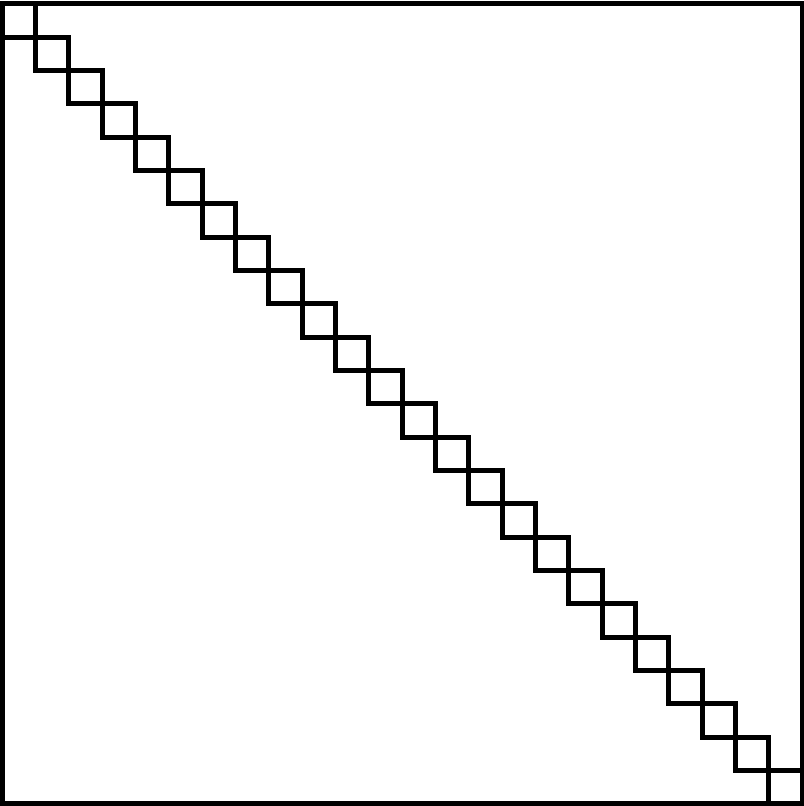
\includegraphics[width=0.18\textwidth]{figura1}\; 
	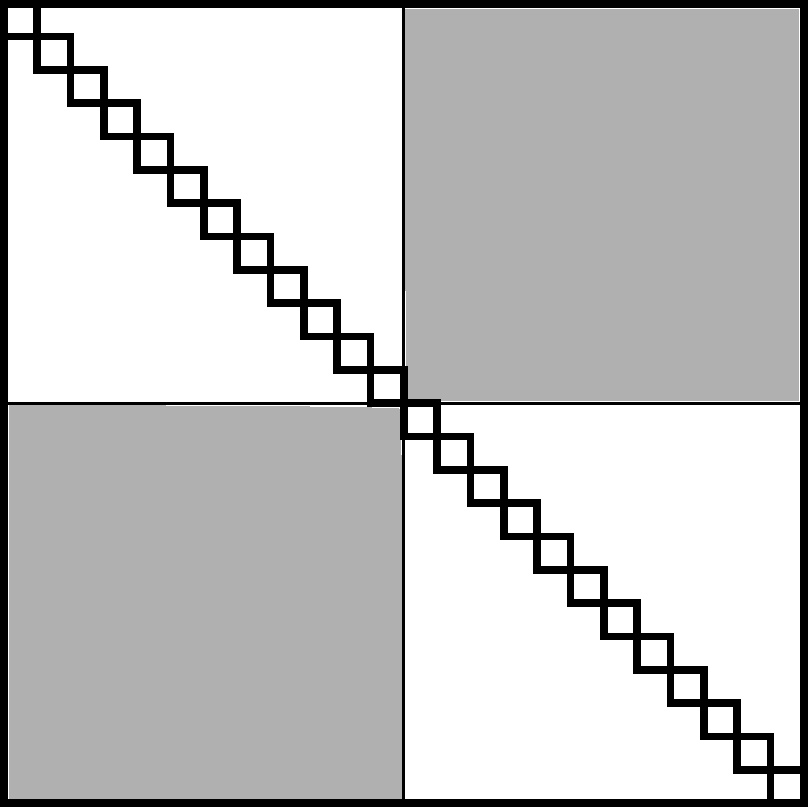
\includegraphics[width=0.18\textwidth]{figura2}\;
	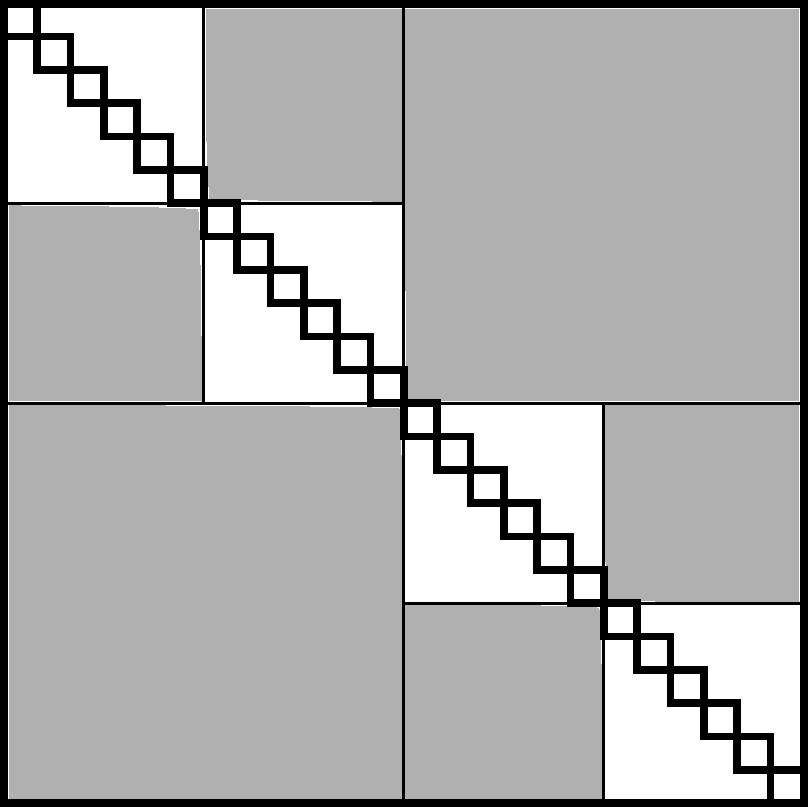
\includegraphics[width=0.18\textwidth]{figura3}\; 
	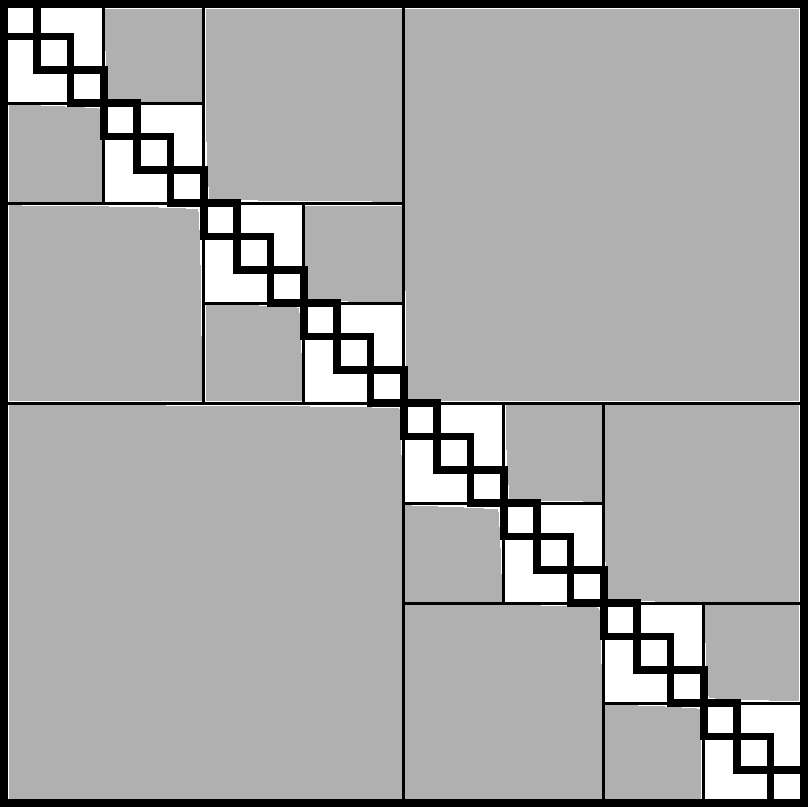
\includegraphics[width=0.18\textwidth]{figura4}\;
	\end{center}

	\begin{itemize}
		\item[\faBox] The \textbf{grey blocks} are \textbf{low rank matrices} represented \textbf{in} a \textbf{compressed form},
		\item[\faBoxOpen] the \emph{diagonal blocks} in the last step are \emph{stored as dense matrices}.
		\item[\faToolbox]<2-> We need now a \textbf{formal definition} and a way to \textbf{define operations}.
	\end{itemize}
	
	\end{frame}

	\begin{frame}{HODLR-matrices: trees}\vspace{-0.3em}
	\begin{block}{\faTree\;Cluster tree}
	Given $n\in \mathbb N$, let $\mathcal T_p$ be a completely balanced binary tree of depth $p$ whose nodes are
	subsets of $\{ 1, \ldots, n \}$. We say that $\mathcal T_p$ is
	a \emph{cluster tree} if it satisfies:
	\begin{itemize}
		\item[\faSeedling]<2-> The root is $I^{0}_1 := I = \{ 1, \ldots, n \}$.
		\item[\faLeaf]<3-> The nodes at level $\ell$, denoted by $I^{\ell}_1, \ldots, I^{\ell}_{2^\ell}$, form
		a partitioning of $\{1, \ldots, n\}$ into consecutive indices:
		\[
		I_i^\ell = \{ n^{(\ell)}_{i-1}+1\ldots, n^{(\ell)}_{i}-1, n_i^{(\ell)} \}
		\]
		for some integers $0 = n^{(\ell)}_{0} \le  n^{(\ell)}_{1} \le \cdots \le n^{(\ell)}_{2^\ell} = n$, $\ell = 0,\ldots p$. In particular, if $n_{i-1}^{(\ell)}=n_i^{(\ell)}$ then $I_i^{\ell}=\emptyset$.
		\item[\faLeaf]<4-> The node $I_{i}^{\ell}$ has children 
		$I_{2i-1}^{\ell+1}$ and $I_{2i}^{\ell+1}$, for any $1 \leq \ell \leq p - 1$. The children form a partitioning of their parent. 
	\end{itemize}
	\end{block}
	\onslide<5>{\faLightbulb\;Nodes at a level $\ell$ partition $A$ into a $2^\ell \times 2^\ell$ block
		matrix with blocks $\{A(I^\ell_i, I^\ell_j)\}_{i,j = 1}^{2^\ell}$.}
	\end{frame}

	\begin{frame}[fragile]{HODLR-matrices: trees}
		
	\begin{center}	
	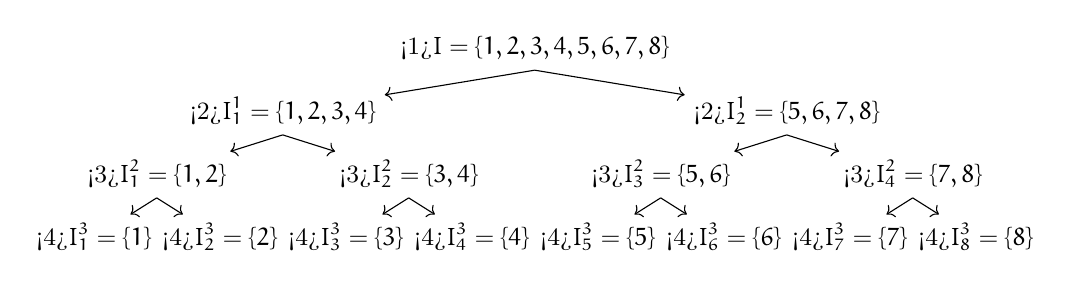
\begin{tikzpicture}[scale=0.8] \small
		\coordinate (T18) at (0,0);  
		\coordinate (T14) at (-4,-1);
		\coordinate (T58) at (4,-1);
		\coordinate (T12) at (-6,-2);
		\coordinate (T34) at (-2,-2);
		\coordinate (T56) at (2,-2);
		\coordinate (T78) at (6,-2);
		\coordinate (T1) at (-7,-3);
		\coordinate (T2) at (-5,-3);
		\coordinate (T3) at (-3,-3);
		\coordinate (T4) at (-1,-3);
		\coordinate (T5) at (1,-3);
		\coordinate (T6) at (3,-3);
		\coordinate (T7) at (5,-3);
		\coordinate (T8) at (7,-3);
		\node (N18) at (T18) {\alert<1>{$I = \{1,2,3,4,5,6,7,8\}$}};
		\node (N14) at (T14) {\alert<2>{$I_1^1 = \{1,2,3,4\}$}};
		\node (N58) at (T58) {\alert<2>{$I_2^1 = \{5,6,7,8\}$}};
		\node (N12) at (T12) {\alert<3>{$I_1^2 = \{1,2\}$}};
		\node (N34) at (T34) {\alert<3>{$I_2^2 = \{3,4\}$}};
		\node (N56) at (T56) {\alert<3>{$I_3^2 = \{5,6\}$}};
		\node (N78) at (T78) {\alert<3>{$I_4^2 = \{7,8\}$}};
		\node (N1) at (T1) {\alert<4>{$I_1^3 = \{1\}$}};
		\node (N2) at (T2) {\alert<4>{$I_2^3 = \{2\}$}};
		\node (N3) at (T3) {\alert<4>{$I_3^3 = \{3\}$}};
		\node (N4) at (T4) {\alert<4>{$I_4^3 = \{4\}$}};
		\node (N5) at (T5) {\alert<4>{$I_5^3 = \{5\}$}};
		\node (N6) at (T6) {\alert<4>{$I_6^3 = \{6\}$}};   
		\node (N7) at (T7) {\alert<4>{$I_7^3 = \{7\}$}};
		\node (N8) at (T8) {\alert<4>{$I_8^3 = \{8\}$}};
		\draw[->] (N18.south) -- (N14);
		\draw[->] (N18.south) -- (N58);  
		\draw[->] (N14.south) -- (N12);
		\draw[->] (N14.south) -- (N34);    
		\draw[->] (N58.south) -- (N56);  
		\draw[->] (N58.south) -- (N78);
		\draw[->] (N12.south) -- (N1);
		\draw[->] (N12.south) -- (N2);
		\draw[->] (N34.south) -- (N3);  
		\draw[->] (N34.south) -- (N4);  
		\draw[->] (N56.south) -- (N5);  
		\draw[->] (N56.south) -- (N6);          
		\draw[->] (N78.south) -- (N7);  
		\draw[->] (N78.south) -- (N8);          
	\end{tikzpicture}
	\end{center}

	\begin{columns}
		\begin{column}{0.7\columnwidth}
\begin{itemize}
\item[\faSeedling]<1-> The root $I = \{1,\ldots,8\}$,
\item[\faLeaf]<2-> Nodes at level $1$: $I_1^1$ and $I_1^2$,
\item[\faLeaf]<3-> Nodes at level $2$: \faLeaf($I_1^1$)$ = \{I_1^2, I_2^2\}$, \faLeaf($I_2^1$)$ = \{I_3^2, I_4^2\}$,
\item[\faLeaf]<4-> Nodes at level $3$:  \faLeaf($I_1^2) = \{I_1^3,I_2^3\}$, $\ldots$, \faLeaf($I_4^2) = \{I_7^3,I_8^3\}$.
\end{itemize}
		\end{column}
		\begin{column}{0.3\columnwidth}
				\begin{onlyenv}<1>
				\begin{tikzpicture}[scale=0.3]    
					\node [above] at (4,8) {$\ell=0$};
					\draw (0,0) -- (0,8) -- (8,8) -- (8,0) -- cycle;
				\end{tikzpicture}
				\end{onlyenv}
				\begin{onlyenv}<2>
				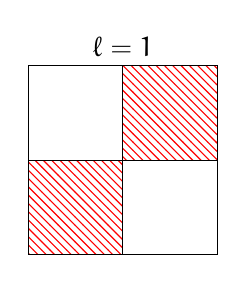
\begin{tikzpicture}[scale=0.3]  
					\node [above] at (4,8) {$\ell=1$};
					\draw (0,0) -- (0,8) -- (8,8) -- (8,0) -- cycle;
					\draw[pattern=north west lines, pattern color=red] (0,0) rectangle (4,4);
					\draw[pattern=north west lines, pattern color=red] (4,4) rectangle (8,8);
					\draw (0,4) -- (8,4);
					\draw (4,0) -- (4,8);
				\end{tikzpicture}
			\end{onlyenv}
				\begin{onlyenv}<3>
				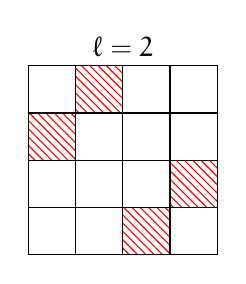
\begin{tikzpicture}[scale=0.3]  
					\node [above] at (4,8) {$\ell=2$};
					\draw (0,0) -- (0,8) -- (8,8) -- (8,0) -- cycle;
					\draw[pattern=north west lines, pattern color=red] (4,0) rectangle (6,2);
					\draw[pattern=north west lines, pattern color=red] (0,4) rectangle (2,6);
					\draw[pattern=north west lines, pattern color=red] (6,2) rectangle (8,4);
					\draw[pattern=north west lines, pattern color=red] (2,6) rectangle (4,8);
					\draw (0,2) -- (8,2);
					\draw (0,4) -- (8,4);
					\draw (0,6) -- (8,6);
					\draw (2,0) -- (2,8);
					\draw (4,0) -- (4,8);
					\draw (6,0) -- (6,8);
				\end{tikzpicture}
			\end{onlyenv}
			\begin{onlyenv}<4>
				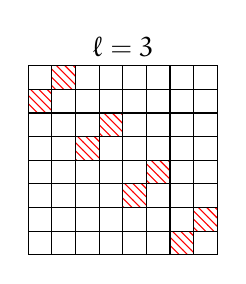
\begin{tikzpicture}[scale=0.3]  
					\node [above] at (4,8) {$\ell=3$};
					\draw (0,0) -- (0,8) -- (8,8) -- (8,0) -- cycle;
					\draw[pattern=north west lines, pattern color=red] (6,0) rectangle (7,1);
					\draw[pattern=north west lines, pattern color=red] (4,2) rectangle (5,3);
					\draw[pattern=north west lines, pattern color=red] (2,4) rectangle (3,5);
					\draw[pattern=north west lines, pattern color=red] (0,6) rectangle (1,7);
					\draw[pattern=north west lines, pattern color=red] (7,1) rectangle (8,2);
					\draw[pattern=north west lines, pattern color=red] (5,3) rectangle (6,4);
					\draw[pattern=north west lines, pattern color=red] (3,5) rectangle (4,6);
					\draw[pattern=north west lines, pattern color=red] (1,7) rectangle (2,8);
					
					\draw (0,1) -- (8,1);
					\draw (0,2) -- (8,2);
					\draw (0,3) -- (8,3);
					\draw (0,4) -- (8,4);
					\draw (0,5) -- (8,5);
					\draw (0,6) -- (8,6);
					\draw (0,7) -- (8,7);
					\draw (1,0) -- (1,8);
					\draw (2,0) -- (2,8);
					\draw (3,0) -- (3,8);
					\draw (4,0) -- (4,8);
					\draw (5,0) -- (5,8);
					\draw (6,0) -- (6,8);
					\draw (7,0) -- (7,8);
				\end{tikzpicture}
			\end{onlyenv}
		\end{column}

	\end{columns}


	
	\end{frame}

	\begin{frame}{HODLR-matrices: definition}

	\begin{block}{HODLR matrix}
	Let $A\in \mathbb{R}^{n\times n}$ and consider a cluster tree $\mathcal T_p$. 
	\begin{enumerate}
		\item Given $k\in \mathbb N$, $A$ is said to be a $(\mathcal T_p,k)$-HODLR matrix if every off-diagonal block
		\begin{equation*}
			A(I_i^\ell,I_j^\ell) \quad \text{such that $I_i^\ell$ and $I_j^\ell$ are siblings in $\mathcal T_p$}, \quad \ell=1,\dots,p,
		\end{equation*} has rank at most $k$.
		\item The HODLR rank of $A$ (with respect to $\mathcal T_p$)  is the smallest integer $k$ such that $A$ is a $(\mathcal T_p,k)$-HODLR matrix.
	\end{enumerate}
	\end{block}

	\begin{itemize}
		\item[\faSeedling]<2-> $\mathcal T_p$ is often chosen to be \alert{as balanced as possible}, i.e., cardinalities of $I^\ell_i$ are nearly equal for a given $\ell$, with a dept determined by a minimal diagonal block
		size $n_{\mathrm{min}}$.
		\item[\faCog]<3-> The classical choice is to have a \textbf{binary tree}, i.e., $n = 2^p n_{\mathrm{min}}$.
	\end{itemize}

	\end{frame}

	\begin{frame}{HODLR-matrices: occupied space}
	If we assume \textbf{identical ranks} $k$ and a \textbf{balanced partitioning} then
	\begin{itemize}
		\item[\faMoneyBillWave] Storage for off-diagonal blocks $A(I_i^\ell,I_j^\ell) = U_i^{(\ell)}(V_j^{(\ell)})^T$, $U_i^{(\ell)},V_j^{(\ell)} \in \mathbb{R}^{m_\ell \times k}$:
		
		On level $\ell > 0$ there are $2^\ell$ off-diagonal blocks
		\[
		2k \sum_{\ell = 1}^{p} 2^\ell m_\ell = 2 k n_0 \sum_{\ell = 1}^{p} 2^\ell 2^{p-\ell} 2 k n_0 p 2^p = 2 k n p = 2 k n \log_2(\nicefrac{n}{n_0}),
		\]
		\item[\faMoneyBillWave]<2-> Storage requirements for diagonal blocks
		\[
		2^p n_0^2 = n n_0, 
		\]
		\item[\faMoneyCheck]<3-> Total, assuming $n_0 = O(1)$, is then
		\[
		O(k n \log n).
		\]
		\item[\faArrowAltCircleDown]<4-> Both \alert{requirements} on ranks and partitioning can be \alert{relaxed to obtain similar results}.
	\end{itemize}
	\end{frame}

	\begin{frame}{HODLR-matrices: building the representation}
		
	\alert{\faExclamationTriangle}\; Is \alert{\textbf{non trivial}} to construct structured representations efficiently, especially if you want to avoid computing the whole $n^2$ coefficients!
	
	\begin{itemize}
		\item[\faSeedling]<2-> Build a \textbf{cluster tree} $\mathcal{T}_p$ for the given index set,
	\end{itemize}
	\onslide<3->{If $A$ is \textbf{dense}:}
	\begin{itemize}
		\item[\faBox]<3-> Use Householder \textbf{QR decomposition} with column pivoting or \textbf{SVD} on off-diagonal blocks,
		\item[\faWrench]<4-> The \textbf{rank} of each off-diagonal block $A(I_i^p, I_j^p)$ is chosen such that the spectral \textbf{norm of the approximation error} is bounded by $\epsilon$ times $\|A(I_i^p, I_j^p)\|_2$.
	\end{itemize}
	\onslide<5->{If $A$ is \textbf{sparse}:}
	\begin{itemize}
		\item[\faBox]<5-> Use a \textbf{two sided Lanczos method} only requiring matrix-vector multiplications with an off-diagonal block and its transpose, combined with recompression to each off-diagonal block. 
	\end{itemize}
	\onslide<6->{If $A$ is \textbf{structured} use an \emph{ad-hoc} constructor!}
	\end{frame}

	\subsection{HODLR of Gr\"unwald--Letnikov}

	\begin{frame}{HODLR of Gr\"unwald--Letnikov}
		
	\begin{alertblock}<1->{Theorem \parencite[Theorem A]{MR2566483}}
	Let $\mathbf x, \mathbf y$ two real vectors of length $N$,
	with ascending and descending ordered entries, respectively.
	Moreover, we denote with  $C(\mathbf x, \mathbf y)$ the Cauchy matrix defined by\vspace{-0.5em}
	\[
	C_{ij} = \frac{1}{x_i - y_j}, \qquad
	i,j = 1, \ldots, N.
	\]
	If $C(\mathbf x, \mathbf y) = C(\mathbf x, \mathbf y)^T$, 
	$x_i \in [a, b]$, $y_j \in [c, d]$ with $a > d$,
	then $C(\mathbf x, \mathbf y)$ is positive definite.
	\end{alertblock}
		
	\begin{alertblock}<2->{Theorem \parencite[Theorem 5.5]{MR3947283}}
		Let $H$ be a positive semidefinite Hankel matrix of size $N$. Then,
	the $\epsilon$-rank of $H$ is bounded by\vspace{-0.5em}
	\[
	\mathrm{rank}_{\epsilon}(H) \leq 2 + 2\left\lceil
	\frac{2}{\pi^2} \log \left( \frac {4}{\pi}N \right)
	\log\left(\frac{16}{\epsilon}\right)
	\right\rceil \triangleq \mathfrak B(N, \epsilon).
	\]
	\end{alertblock}
	
	\end{frame}

	\begin{frame}{HODLR of Gr\"unwald--Letnikov}
	We need to work with $G_N \in \mathbb{R}^{N \times N}$
	\begin{columns}
	\begin{column}{0.55\columnwidth}
	\begin{equation*}
		G_{N}= -\left[
		\begin{matrix}
			g_1^{(\alpha)}& g_0^{(\alpha)} & 0 & \cdots & 0 &0\\
			g_2^{(\alpha)}& g_1^{(\alpha)} & g_0^{(\alpha)}& 0 &\cdots & 0\\
			\vdots &\ddots & \ddots & \ddots &\ddots & \vdots\\
			\vdots &\ddots & \ddots & \ddots &\ddots & 0\\
			g_{N-1}^{(\alpha)}&\ddots & \ddots & \ddots & g_1^{(\alpha)}& g_0^{(\alpha)}\\
			g_{N}^{(\alpha)}& g_{N-1}^{(\alpha)} & \cdots & \cdots & g_2^{(\alpha)}& g_1^{(\alpha)}
		\end{matrix}
		\right]
	\end{equation*}
	\end{column}
	\begin{column}{0.45\columnwidth}
	\begin{alertblock}{Lemma \parencite{MR3995304}}
	Consider the Hankel matrix $H$ defined as
	\[
	H = (h_{ij}), \qquad
	h_{ij} = g_{i+j}^{(\alpha)},
	\]
	for $1 \leq \alpha \leq 2$. Then, $H$ is positive semidefinite.
	\end{alertblock}
	\end{column}
	\end{columns}
	\vfill

	\faHammer\; Show that $H$ is obtained as the sum of a positive definite Cauchy matrix and a positive semidefinite matrix.\vfill
	
	\faHammer\; Use the result by \cite{MR3947283}.

	\end{frame}

	\begin{frame}{HODLR of Gr\"unwald--Letnikov}
	\textbf{Proof}. For $k\geq 2$ we rewrite $g_{k}^{(\alpha)}$ as
	\begin{align*}
	g_{k}^{(\alpha)} \only<1>{&= \frac{(-1)^k}{k!} \alpha (\alpha - 1) \ldots (\alpha - k + 1) \\
	&= \frac{\alpha (\alpha - 1)}{k!} (k-\alpha-1) (k-\alpha-2) \ldots (2 - \alpha) \\}
	&= \alpha (\alpha - 1) \frac{\Gamma(k-\alpha)}{\Gamma(k+1) \Gamma(2-\alpha)}.
\end{align*}
	\only<2>{ Use the Gauss representation of the Euler $\Gamma$
	\[
		\Gamma(z) = \lim_{m \to \infty} \frac{m! m^z}{z (z + 1) (z + 2) \ldots (z+m)}, \quad
	z \neq \{ 0, -1, -2, \ldots \},
	\]
	we rewrite
	\[
	g_{k}^{(\alpha)} = \alpha (\alpha - 1) \lim_{m \to \infty} \frac{1}{m! m^3} \prod_{p = 0}^{m} \frac{k+1+p}{k-\alpha+p} (2 - \alpha + p).
	\]
	}\only<3->{
	We rewrite
	\[
	H = \lim_{m \rightarrow + \infty} H_0 \circ \ldots \circ H_{m}, \qquad (H_p)_{ij} = \frac{i+j+1+p}{i+j-\alpha+p}
	\]
	for $\circ$ the Hadamard product, $\{H_j\}_{j=0}^{m}$ Hankel matrices. \only<4>{\alert{Schur Product Theorem} tells us that ``\emph{the Hadamard product of two positive definite matrices is also a positive definite matrix}'' $\Rightarrow$ If $H_0 \circ \ldots \circ H_{m}$ is positive semidefinite for every $m$ then $H$ is also
	positive semidefinite.}\only<5->{Rewrite
	\[
	(H_p)_{ij} = \only<5>{\frac{i+j+1+p}{i+j-\alpha+p} =} 1 + \frac{\alpha+1}{i+j-\alpha+p} \onslide<6->{,\quad H_p = \boldsymbol{1} \boldsymbol{1}^T +
		(\alpha + 1) \cdot C(\mathbf x, - \mathbf x), \quad
		\mathbf x =
		\begin{bmatrix}
			1 \\
			\vdots \\
			N
		\end{bmatrix}  + \frac{p-\alpha}{2} \boldsymbol{1},}
	\]
	}
	\only<6>{ $\mathbf{x} \geq 0$ for $\alpha < 2$, thus $C(\mathbf{x},-\mathbf{x})$ is PD. Then $H_p$ is positive semidefinite as the sum of a PD and positive semidefinite matrix. \hfill \qed}
	}
	\end{frame}

	\begin{frame}[fragile]{HODLR of Gr\"unwald--Letnikov}
	
	\begin{onlyenv}<1-5,8->\begin{alertblock}{Proposition \parencite[Lemma 3.15]{MR3995304}}
	For every $\epsilon > 0$, the $\epsilon$-qsrank of $G_N$
	is bounded by\vspace{-0.5em}
	\[
	\operatorname{qsrank}_{\epsilon} (G_N)
	\leq \mathfrak B\left(N, \frac{\epsilon}{2}\right) =
	2 + 2\left\lceil
	\frac {2}{\pi^2} \log \left( \frac{4}{\pi}N \right)
	\log\left(\frac{32}{\epsilon}\right)
	\right\rceil.
	\]
	\end{alertblock}\end{onlyenv}
	\begin{onlyenv}<6,7>
	\begin{columns}
	\begin{column}{0.45\columnwidth}
	\begin{onlyenv}<6>\centering
	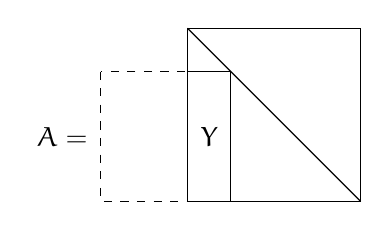
\begin{tikzpicture}[scale=0.55]
		\node at (-2.9,1.5) { $A = $} ;
		\draw (0,0) rectangle (4,4);
		\draw (0,4) -- (4,0);
		\draw (0,3) -- (1,3) -- (1,0);
		%	\draw (0,2) -- (1,2);
		\draw[dashed] (-2,3) rectangle (0,0);
		%	\draw[dashed] (-2,2) -- (0,2);
		%	\node at (.5,2.5) { $Y_1$ };
		\node at (.5,1.5) {  $Y$ };
		%	\node at (.5,1) { $Y_2$ };
		\node at (-1,1) {  };
	\end{tikzpicture}
	\end{onlyenv}
	\begin{onlyenv}<7>
		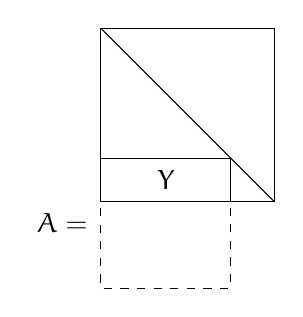
\begin{tikzpicture}[scale=0.55]
		\node at (-0.9,-.5) { $A = $} ;
		\draw (0,0) rectangle (4,4);
		\draw (0,4) -- (4,0);
		\draw (0,1) -- (3,1) -- (3,0);
		%	\draw (0,2) -- (1,2);
		\draw[dashed] (0,1) rectangle (3,-2);
		%	\draw[dashed] (-2,2) -- (0,2);
		%	\node at (.5,2.5) { $Y_1$ };
		\node at (1.5,.5) {  $Y$ };
		%	\node at (.5,1) { $Y_2$ };
		\node at (-1,1) {  };
	\end{tikzpicture}
	\end{onlyenv}
	\end{column}
	\begin{column}{0.53\columnwidth}
	For every $1 \leq i \leq s$ and 
	$1 \leq j \leq t$ one have $Y_{ij} = -g_{1+i-j+t}^{(\alpha)} = -g_{1+i-(j-t+h)+h}^{(\alpha)} = A_{i,j-t+h}$.
	\end{column}
	\end{columns}
	\end{onlyenv}

	\textbf{Proof.} \only<2>{We just need to work on the lower triangle, for the upper the rank is at most $1$ (Hessenberg).}\only<3->{Let $Y \in \mathbb R^{s \times t}$ 
		be any lower off-diagonal block of $G_N$. \emph{Without loss of generality} we assume that $Y$ is maximal, i.e. $s+t=N$.}\only<4>{ (If $\mathrm{rank}(Y+\delta Y)=k$ and $\|\delta Y\|_2\leq \epsilon\|G_N\|_2$ then the submatrices of $\delta Y$ verify the analogous claim for the corresponding ones of $Y$.)}
	
	\only<5->{Entries $Y$ are given by $Y_{ij} = -g_{1+i-j+t}^{(\alpha)}$. Call $h = \max\{s, t\}$, and $A$ the $h \times h$ matrix defined by $A_{ij} = -g_{1+i-j+h}^{(\alpha)}$.}\only<6->{$Y$ coincides with  either the last $t$ columns or the first $s$ rows of $A$.}\only<8->{ In particular,
		$Y$ is a submatrix of $A$ and therefore $\|{Y}\|_2 \leq \|A\|_2$.} \only<9>{\faCog\; We need now to estimate $\|A\|_2$ in terms of $\|G_N\|_2$, thus we partition
	\[
	A=\begin{bmatrix}A^{(11)}&A^{(12)}\\ A^{(21)}& A^{(22)}\end{bmatrix}, \qquad A^{(ij)}\in\mathbb C^{m_{ij}\times n_{ij}},\qquad 
	\begin{cases}
		m_{1j}=n_{i1}=\lceil\frac h2\rceil \\
		m_{2j}=n_{i2}=\lfloor\frac h2\rfloor
	\end{cases}, \quad \begin{cases}
	h \leq N-1, \\ m_{i,j} + n_{i,j} \leq N,
\end{cases}
	\]}
	
	\end{frame}

	\begin{frame}{HODLR of Gr\"unwald--Letnikov}
	\textbf{Proof.} \only<1->{and consider 
	the subdiagonal block $T^{(ij)}$ of 
	$G_N$ defined by
	\[
	T^{(ij)} = G_N(N-m_{ij}+1:N, N-m_{ij}-n_{ij}+1:N-m_{ij}), \qquad 
	i,j = 1,2, \quad \begin{array}{l}T^{(ij)} \in \mathbb{R}^{m_{ij}\times n_{ij}}, \\ m_{ij} + n_{ij} \leq N.\end{array}
	\]
	\begin{itemize}
	\item[\faEye]<2-> Since $g_j^{(\alpha)}>g_{j+1}^{(\alpha)}>0$, $|T^{(ij)}| \geq |A^{(ij)}|$ for 
	every $i,j = 1,2$,
	\item[\faHammer]<3-> Being $T^{(ij)}$ and $A^{(ij)}$ 
	nonpositive and the $2$ norm monotonous, $\|A^{(ij)}\|_2 \leq \|T^{(ij)}\|_2$.
	\item[\faLightbulb]<4-> By exploiting
	\[
	\begin{array}{ll}
		\|{A}\|_2 &\leq \left\lVert\begin{bmatrix}A^{(11)}&\\ & A^{(22)}\end{bmatrix}\right\rVert_2 +\left\lVert\begin{bmatrix}&A^{(12)}\\ A^{(21)}& \end{bmatrix}\right\rVert_2 \\[1em]
		&= \max\{\|{A^{(11)}}\|_2,\|{A^{(22)}}\|_2\} +\max\{\|{A^{(12)}}\|_2,\|{A^{(21)}}\|_2\} 
	\end{array}	\; \Rightarrow \; \|A\|_2 \leq 2 \|G_N\|_2.
	\]
	\item[\faBomb]<5-> Conclude by the result on Hankel matrices!
	\end{itemize}

	}
	\end{frame}

	\begin{frame}{HODLR of Gr\"unwald--Letnikov}
	\begin{alertblock}{Proposition \parencite[Lemma 3.15]{MR3995304}}
		For every $\epsilon > 0$, the $\epsilon$-qsrank of $G_N$
		is bounded by\vspace{-0.5em}
		\[
		\operatorname{qsrank}_{\epsilon} (G_N)
		\leq \mathfrak B\left(N, \frac{\epsilon}{2}\right) =
		2 + 2\left\lceil
		\frac {2}{\pi^2} \log \left( \frac{4}{\pi}N \right)
		\log\left(\frac{32}{\epsilon}\right)
		\right\rceil.
		\]
	\end{alertblock}

	\textbf{Proof.} We call $J$ the $h \times h$ flip matrix, so that $-AJ$ is Hankel and positive semidefinite:
	\[
	\mathrm{rank}_{\frac \epsilon 2}(A) = \mathrm{rank}_{\frac \epsilon 2}(AJ) \leq \mathfrak B\left(N, \frac \epsilon 2\right).
	\]
	\onslide<2->{$Y$ is a submatrix of $A$, thus there exists $\delta Y$ such that
	\[
	\|\delta Y\|_2 \leq \varepsilon \|G_N\|_2 \text{ and }\mathrm{rank}(Y+\delta Y)\leq \mathfrak B\left(N, \frac \epsilon 2\right).
	\]
	}\onslide<3>{$\Rightarrow$ $\mathrm{qsrank}_{\epsilon}(G_N) \leq \mathfrak B\left(N, \frac \epsilon 2\right)$. \hfill \qed}
	\end{frame}

	\begin{frame}[fragile]{HODLR of Gr\"unwald--Letnikov}
	Let's do some experiments with the \href{https://github.com/numpi/hm-toolbox}{\faGithub}\,\texttt{hm-toolbox}~\parencite{MR4082285}.
	
	\begin{columns}
	\begin{column}{0.6\columnwidth}
\definecolor{bg}{rgb}{0.95,0.95,0.95}
\begin{minted}[bgcolor=bg,fontsize=\small,breaklines]{matlab}
function G = glhodlrmatrix(N,alpha,tol)
%%GLMATRIX produces the GL discretization of 
% the Riemann-Liouville derivative in HODLR 
% format
g = gl(N,alpha);
c = zeros(N,1);
r = zeros(1,N);
r(1:2) = g(2:-1:1);
c(1:N) = g(2:end);
hodlroption( 'threshold', tol);
G = hodlr('toeplitz',c,r);
end
\end{minted}
	\end{column}
	\begin{column}{0.45\columnwidth}
\centering
\only<2>{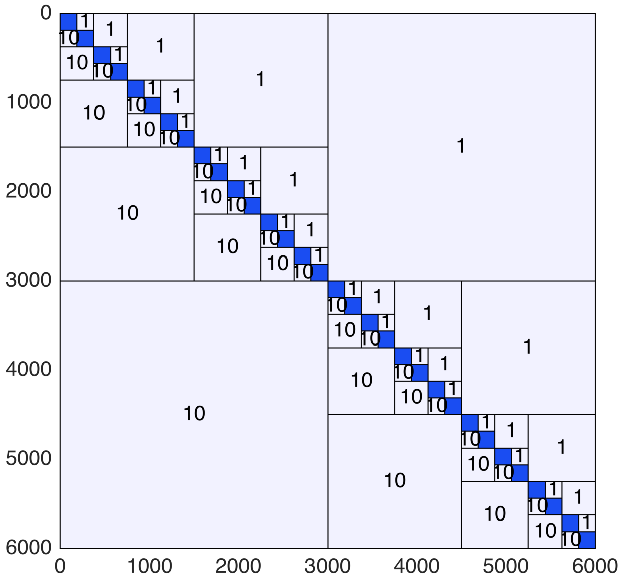
\includegraphics[width=0.8\columnwidth]{hodlrgl1.pdf}}%
\only<3>{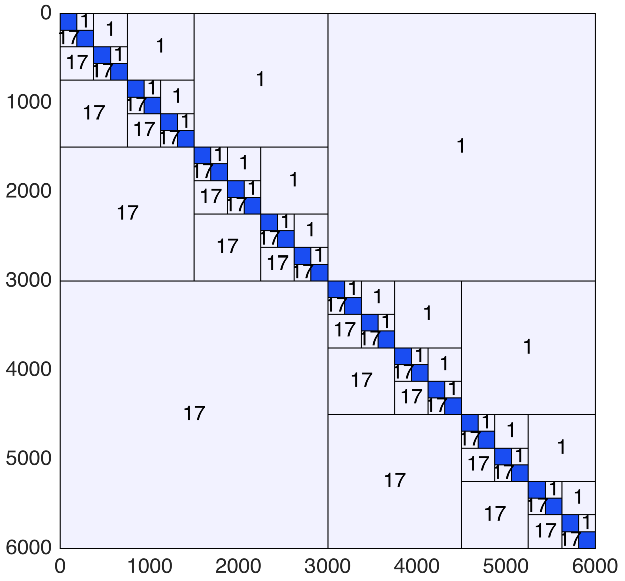
\includegraphics[width=0.8\columnwidth]{hodlrgl2.pdf}}%
\only<4>{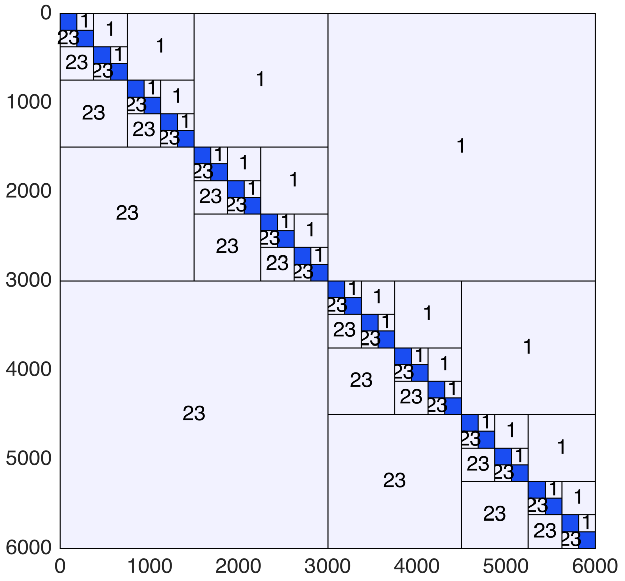
\includegraphics[width=0.8\columnwidth]{hodlrgl3.pdf}}%
\begin{onlyenv}<2>
\definecolor{bg}{rgb}{0.95,0.95,0.95}
\begin{minted}[bgcolor=bg,fontsize=\footnotesize,breaklines]{matlab}
G = glhodlrmatrix(6000,1.5,1e-6);
\end{minted}
\end{onlyenv}
\begin{onlyenv}<3>
\definecolor{bg}{rgb}{0.95,0.95,0.95}
\begin{minted}[bgcolor=bg,fontsize=\footnotesize,breaklines]{matlab}
G = glhodlrmatrix(6000,1.5,1e-9);
\end{minted}
\end{onlyenv}
\begin{onlyenv}<4>
\definecolor{bg}{rgb}{0.95,0.95,0.95}
\begin{minted}[bgcolor=bg,fontsize=\footnotesize,breaklines]{matlab}
G = glhodlrmatrix(6000,1.5,1e-12);
\end{minted}
\end{onlyenv}
	\end{column}
	\end{columns}
	
	
	\end{frame}

	\begin{frame}{HODLR Matrix: the whole discretization}
	Matrix $G_N$ was only a piece of the whole discretization matrix
	\[
	A_N = I_N + \frac{\Delta t}{h^\alpha} \left(D^+_{(m)} G_N + D^-_{(m)} G_N^T\right),
	\]
	does it share the same structure?
	
	\begin{alertblock}<2->{Corollary \parencite[Corollary 3.16]{MR3995304}}
\[
\mathrm{qsrank}_{\epsilon}(A_N) \leq
3 + 2\left\lceil
\frac 2{\pi^2} \log \left( \frac{4}{\pi}N \right)
\log\left(\frac{32}{\hat\epsilon}\right)
\right\rceil, \quad
\hat\epsilon \triangleq \frac{\|A_N\|}{\|G_N\| \cdot \max\{\|D^+_{(m)}\|, \|D^-_{(m)}\|\}} \epsilon.
\]
	\end{alertblock}
\only<3->{\textbf{Proof.} Result is invariant under scaling, so assume wlog that 
	$\frac{\Delta t}{h^\alpha} = 1$. \only<4>{A generic off-diagonal block $Y$, wlog in the lower
		triangular part, If $Y$ does not intersect the first
		subdiagonal, is a subblock of $D^+_{(m)} G_N$, so there
		exists a perturbation
		$\delta Y$
		with norm bounded by $\|{\delta Y}\| \leq \|{D^+_{(m)}}\| \|{G_N}\| \cdot \hat\epsilon$ such that $Y + \delta Y$ has rank at most $\mathfrak B(N, \nicefrac{\hat\epsilon}{2})$.
		In particular, $\delta Y$ satisfies $\|{\delta Y}\| \leq \|{A_N}\| \cdot \epsilon$. }\only<5->{Since we have excluded one subdiagonal, a generic off-diagonal
		block $Y$ we can find a perturbation with norm bounded
		by $\|{A_N}\| \cdot \epsilon$ such that $Y + \delta Y$
		has rank $1 + \mathfrak{B}(N, \nicefrac{\hat\epsilon}{2})$. \hfill \qed}

}
	
	\end{frame}

	\begin{frame}[fragile]{A HODLR right-hand side}
	\faQuestionCircle\;What are right-hand sides functions $f(x,y,t)$ so that the matrix C has a HODLR structure?\vspace{1em}
	
	\begin{columns}
	\begin{column}{0.5\columnwidth}
	\onslide<2->{
	Consider the function\vspace{-1em}
	\[
	f(x,y) = \log \left( \tau + \left| x - y \right| \right), \quad \tau > 0.
	\]}\vspace{-2em}
	\begin{itemize}
		\item[\faCog]<3-> If we discretize it by \emph{finite differences} on a rectangular domain we find
		\[
		C_{i,j}= \log \left( \tau + \left| x_i - y_j \right| \right)
		\]
		\item[\faLightbulb]<4-> The modulus function it is
		\textbf{not regular in the whole domain} \alert{but} it is \textbf{analytic} when the \textbf{sign} of
		$x-y$ is \textbf{constant}.
		\item[\faHammer]<5-> We can use again Chebyshev basis to approximate it in a separable fashion. 
	\end{itemize}
	\end{column}
	\begin{column}{0.5\columnwidth}\centering
	\only<2-4>{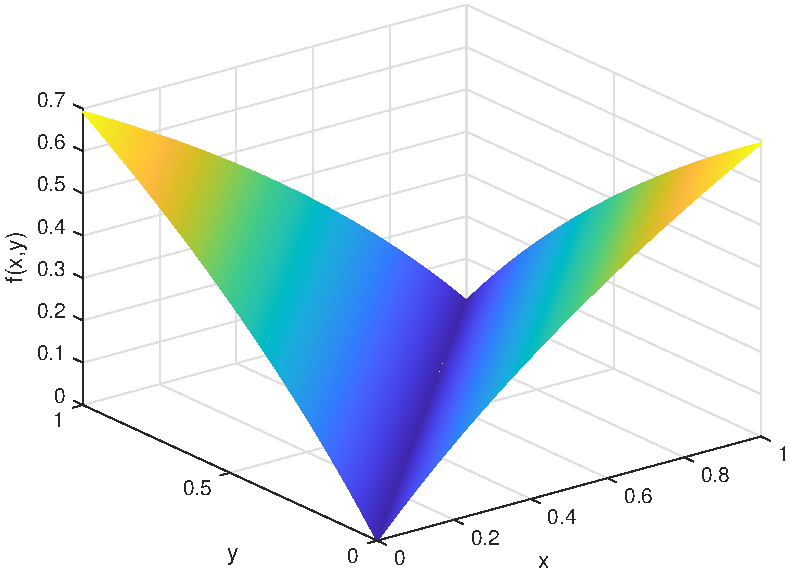
\includegraphics[width=0.8\columnwidth]{rhs1.pdf}}%
	\only<5>{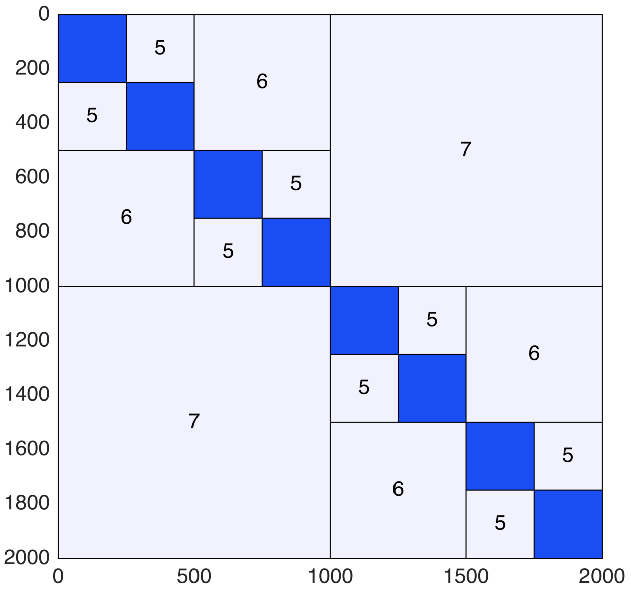
\includegraphics[width=0.6\columnwidth]{rhs2.pdf}}
	
	\begin{onlyenv}<5->
\definecolor{bg}{rgb}{0.95,0.95,0.95}
\begin{minted}[bgcolor=bg,fontsize=\footnotesize,breaklines]{matlab}
x = linspace(0,1,N); y = linspace(0,1,N);
[X,Y] = meshgrid(x,y); tau = 1;
C = log(tau + abs(X-Y)); hC = hodlr(C);
\end{minted}
	\end{onlyenv}
	\end{column}
	\end{columns}
	
	\end{frame}

	\begin{frame}{Separability (a bit more formally)}
	
	\begin{alertblock}{Separable expansion~\parencite[Definition 4.4]{MR3445676}}
	Take a function $\chi(x,y) : X \times Y \rightarrow \mathbb{R}$, we call 
	\[
	\chi(x,y) = \sum_{\nu = 1}^{r} \phi_\nu^{(r)}(x) \psi_{\nu}^{(r)}(y) + R_r(x,y), \qquad \text{for }x \in X,\,y \in Y,
	\]
	a \emph{separable expansion} of $\chi$ with $r$ terms in $X \times Y$ with remainder $R_r$.
	\end{alertblock}
	\begin{itemize}
		\item[\faWrench]<1-> To have an idea of the \textbf{goodness} of the \emph{separable expansion}, we would like to have $\{\|R_r\|_{\infty},\|R_r\|_{\mathbb{L}^p}\} \overset{r \rightarrow 0}{\longrightarrow} 0$ \alert{as fast as possible}, e.g., \textbf{exponentially}.
		\item[\faCog]<2-> If $\|R_r\| \leq c_1 \exp( - c_2 r^\alpha)$ $\Rightarrow$ $\| R_r \| \leq \varepsilon$ if $r \geq \left\lceil \left( \frac{1}{c_2} \log^{\nicefrac{1}{\alpha}} \frac{c_1}{\varepsilon} \right) \right\rceil = O( \log^{\nicefrac{1}{\alpha}} \nicefrac{1}{\varepsilon} )$ $\varepsilon \rightarrow 0$.
		\item[\faHammer]<3-> We can use Taylor expansions, Chebyshev expansion, Hermite/Lagrange interpolation, cross approximation$\ldots$ In all the cases, the behavior of $R_r$ is tied to the regularity of $\chi(x,y)$; see~\parencite[Chapter~4]{MR3445676}.
	\end{itemize}
	
	\end{frame}

	\subsection{BLAS with HODLR format}

	\begin{frame}{BLAS with HODLR format}
	\faQuestionCircle\;We now have \textbf{everything represented in the right format}, but can we operate with it?
	
	\begin{description}
		\item[$\mathbf{y} = A\mathbf{x}$:]<2-> Matrix-vector products, \emph{recursively}:
		\[
		\begin{array}{l}
			\mathbf{y}(I^1_1) = A(I_1^1,I_1^1) \mathbf{x}(I_1^1) + A(I^1_1,I_2^1) \mathbf{x}(I_2^1),\\
			\mathbf{y}(I^1_2) = A(I_2^1,I_1^1) \mathbf{x}(I_1^1) + A(I^1_2,I_2^1) \mathbf{x}(I_2^1).\\
		\end{array}
		\]
		\begin{itemize}
			\item[\faCog]<3-> Off-diagonal blocks $A(I_1^1,I_2^1)$ and $A(I_2^1,I_1^1)$ are obtained by multiplying $\nicefrac{n}{2} \times \nicefrac{n}{2}$ low-rank matrix with vector. This \alert{\textbf{cost}} $c_{\text{LR}\cdot\mathbf{x}}(\nicefrac{n}{2}) = 2nk$.
			\item[\faCog]<4-> Diagonal blocks are processed recursively at a \alert{\textbf{cost}}
			\[
			c_{A\cdot \mathbf{x}}(n) = 2 c_{A\cdot \mathbf{x}}(\nicefrac{n}{2}) + 4kn + n.
			\]
		\end{itemize}
		\onslide<5->{\textbf{Master theorem} (\emph{divide and conquer}): $c_{A\cdot \mathbf{x}}(n) = (4k+1) \log_2(n) n$.}
	\end{description}
	
	\end{frame}

	\begin{frame}{BLAS with HODLR format}
	\begin{description}
		\item[$C = A + B$:] Adding two equally partitioned HODLR matrices \textbf{increases the ranks} of off-diagonal blocks by a factor $2$.
		\begin{itemize}
			\item[\faCog]<2-> We need truncation $\mathfrak{T}_k( A(I_1^\ell,I_j^\ell) + B(I_1^\ell,I_j^\ell) )$, costs
			\[
			c_{\text{LR}+\text{LR}} = c_{\text{SVD}} \times (n k^2 + k^3),
			\]
		where $c_{\text{SVD}}$ is the cost of the given low-rank truncation algorithm (SVD, rand-SVD, QR, $\ldots$)
		\end{itemize}
		\onslide<3->{Total cost is then:
		\[
		\begin{split}
		\sum_{\ell=1}^p 2^\ell c_{\text{LR}+\text{LR}}(m_\ell) = & c_{\text{SVD}}  \sum_{\ell = 1}^{p} 2^\ell (k^3 + m_\ell k^2) \\
		\leq & c_{\text{SVD}} \left( 2^{p+1} k^3 + \sum_{\ell = 1}^p 2^\ell 2^{p-\ell} n_0 k^2 \right) \\
		\leq & c_{\text{SVD}} \left( 2nk^3 + n \log_2(n)k^2 \right).
		\end{split}
		\]
	
	}
	\end{description}
	\end{frame}

	\begin{frame}[fragile]{BLAS with HODLR format}
	\begin{description}
		\item[$C=AB$:] Matrix-matrix multiplication can also be done recursively
		\[
		\vcenter{\hbox{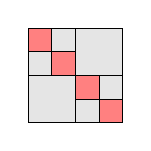
\begin{tikzpicture}[scale=0.6]
		% outerblock
		\draw[fill=gray!20,draw=black] (0,0) rectangle (1,1);
		\draw[fill=gray!20,draw=black] (1,0) rectangle (2,1);
		\draw[fill=gray!20,draw=black] (0,-1) rectangle (1,0);
		\draw[fill=gray!20,draw=black] (1,-1) rectangle (2,0);
		%inblocks (1,1)
		\draw[fill=red!50,draw=black] (0,0.5) rectangle (0.5,1);
		\draw[fill=red!50,draw=black] (0.5,0) rectangle (1,0.5);
		%inblocks (2,2)
		\draw[fill=red!50,draw=black] (1,-0.5) rectangle (1.5,0);
		\draw[fill=red!50,draw=black] (1.5,-1) rectangle (2,-0.5);
		\end{tikzpicture}}} \cdot 		\vcenter{\hbox{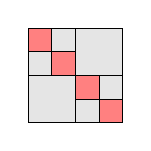
\begin{tikzpicture}[scale=0.6]
		% outerblock
		\draw[fill=gray!20,draw=black] (0,0) rectangle (1,1);
		\draw[fill=gray!20,draw=black] (1,0) rectangle (2,1);
		\draw[fill=gray!20,draw=black] (0,-1) rectangle (1,0);
		\draw[fill=gray!20,draw=black] (1,-1) rectangle (2,0);
		%inblocks (1,1)
		\draw[fill=red!50,draw=black] (0,0.5) rectangle (0.5,1);
		\draw[fill=red!50,draw=black] (0.5,0) rectangle (1,0.5);
		%inblocks (2,2)
		\draw[fill=red!50,draw=black] (1,-0.5) rectangle (1.5,0);
		\draw[fill=red!50,draw=black] (1.5,-1) rectangle (2,-0.5);
	\end{tikzpicture}}} = \begin{bmatrix}
\vcenter{\hbox{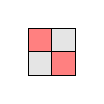
\begin{tikzpicture}[scale=0.6]
\draw[fill=gray!20,draw=black] (0,0) rectangle (1,1);
\draw[fill=red!50,draw=black] (0,0.5) rectangle (0.5,1);
\draw[fill=red!50,draw=black] (0.5,0) rectangle (1,0.5);
\end{tikzpicture}}} \cdot \vcenter{\hbox{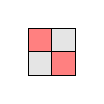
\begin{tikzpicture}[scale=0.6]
\draw[fill=gray!20,draw=black] (0,0) rectangle (1,1);
\draw[fill=red!50,draw=black] (0,0.5) rectangle (0.5,1);
\draw[fill=red!50,draw=black] (0.5,0) rectangle (1,0.5);
\end{tikzpicture}}} + \vcenter{\hbox{
\begin{tikzpicture}[scale=0.6]
\draw[fill=gray!20,draw=black] (0,0) rectangle (1,1);
\end{tikzpicture}}} \cdot \vcenter{\hbox{
\begin{tikzpicture}[scale=0.6]
\draw[fill=gray!20,draw=black] (0,0) rectangle (1,1);
\end{tikzpicture}}} & \vcenter{\hbox{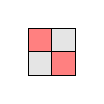
\begin{tikzpicture}[scale=0.6]
\draw[fill=gray!20,draw=black] (0,0) rectangle (1,1);
\draw[fill=red!50,draw=black] (0,0.5) rectangle (0.5,1);
\draw[fill=red!50,draw=black] (0.5,0) rectangle (1,0.5);
\end{tikzpicture}}} \cdot \vcenter{\hbox{
\begin{tikzpicture}[scale=0.6]
\draw[fill=gray!20,draw=black] (0,0) rectangle (1,1);
\end{tikzpicture}}} + \vcenter{\hbox{
\begin{tikzpicture}[scale=0.6]
\draw[fill=gray!20,draw=black] (0,0) rectangle (1,1);
\end{tikzpicture}}} \cdot \vcenter{\hbox{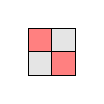
\begin{tikzpicture}[scale=0.6]
\draw[fill=gray!20,draw=black] (0,0) rectangle (1,1);
\draw[fill=red!50,draw=black] (0,0.5) rectangle (0.5,1);
\draw[fill=red!50,draw=black] (0.5,0) rectangle (1,0.5);
\end{tikzpicture}}} \\[1em]
\vcenter{\hbox{
\begin{tikzpicture}[scale=0.6]
\draw[fill=gray!20,draw=black] (0,0) rectangle (1,1);
\end{tikzpicture}}} \cdot \vcenter{\hbox{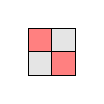
\begin{tikzpicture}[scale=0.6]
\draw[fill=gray!20,draw=black] (0,0) rectangle (1,1);
\draw[fill=red!50,draw=black] (0,0.5) rectangle (0.5,1);
\draw[fill=red!50,draw=black] (0.5,0) rectangle (1,0.5);
\end{tikzpicture}}} + \vcenter{\hbox{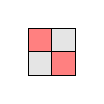
\begin{tikzpicture}[scale=0.6]
\draw[fill=gray!20,draw=black] (0,0) rectangle (1,1);
\draw[fill=red!50,draw=black] (0,0.5) rectangle (0.5,1);
\draw[fill=red!50,draw=black] (0.5,0) rectangle (1,0.5);
\end{tikzpicture}}} \cdot \vcenter{\hbox{
\begin{tikzpicture}[scale=0.6]
\draw[fill=gray!20,draw=black] (0,0) rectangle (1,1);
\end{tikzpicture}}} & \vcenter{\hbox{
\begin{tikzpicture}[scale=0.6]
\draw[fill=gray!20,draw=black] (0,0) rectangle (1,1);
\end{tikzpicture}}} \cdot \vcenter{\hbox{
\begin{tikzpicture}[scale=0.6]
\draw[fill=gray!20,draw=black] (0,0) rectangle (1,1);
\end{tikzpicture}}} + \vcenter{\hbox{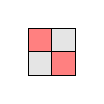
\begin{tikzpicture}[scale=0.6]
\draw[fill=gray!20,draw=black] (0,0) rectangle (1,1);
\draw[fill=red!50,draw=black] (0,0.5) rectangle (0.5,1);
\draw[fill=red!50,draw=black] (0.5,0) rectangle (1,0.5);
\end{tikzpicture}}} \cdot \vcenter{\hbox{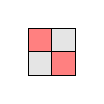
\begin{tikzpicture}[scale=0.6]
\draw[fill=gray!20,draw=black] (0,0) rectangle (1,1);
\draw[fill=red!50,draw=black] (0,0.5) rectangle (0.5,1);
\draw[fill=red!50,draw=black] (0.5,0) rectangle (1,0.5);
\end{tikzpicture}}} 
\end{bmatrix} 
		\]
	where 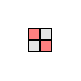
\begin{tikzpicture}[scale=0.3]
	\draw[fill=gray!20,draw=black] (0,0) rectangle (1,1);
	\draw[fill=red!50,draw=black] (0,0.5) rectangle (0.5,1);
	\draw[fill=red!50,draw=black] (0.5,0) rectangle (1,0.5);
\end{tikzpicture} is a $\nicefrac{n}{2}\times \nicefrac{n}{2}$ HODLR matrix and 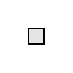
\begin{tikzpicture}[scale=0.2]
	\draw[fill=gray!20,draw=black] (0,0) rectangle (1,1);
\end{tikzpicture} is a low-rank block.		
\end{description}
\begin{multicols}{2}
\begin{enumerate}
	\item<2->  $ \vcenter{\hbox{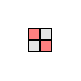
\begin{tikzpicture}[scale=0.3]
				\draw[fill=gray!20,draw=black] (0,0) rectangle (1,1);
				\draw[fill=red!50,draw=black] (0,0.5) rectangle (0.5,1);
				\draw[fill=red!50,draw=black] (0.5,0) rectangle (1,0.5);
	\end{tikzpicture}}} \cdot \vcenter{\hbox{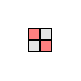
\begin{tikzpicture}[scale=0.3]
	\draw[fill=gray!20,draw=black] (0,0) rectangle (1,1);
	\draw[fill=red!50,draw=black] (0,0.5) rectangle (0.5,1);
	\draw[fill=red!50,draw=black] (0.5,0) rectangle (1,0.5);
\end{tikzpicture}}} $  $\cdot$ of 2 HODLR $\nicefrac{n}{2}$ matrices,
\item<3-> $ \vcenter{\hbox{
\begin{tikzpicture}[scale=0.3]
			\draw[fill=gray!20,draw=black] (0,0) rectangle (1,1);
\end{tikzpicture}}} \cdot \vcenter{\hbox{
\begin{tikzpicture}[scale=0.3]
			\draw[fill=gray!20,draw=black] (0,0) rectangle (1,1);
\end{tikzpicture}}} $ $\cdot$ of 2 low-rank blocks,
\item<4-> $ \vcenter{\hbox{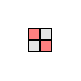
\begin{tikzpicture}[scale=0.3]
			\draw[fill=gray!20,draw=black] (0,0) rectangle (1,1);
			\draw[fill=red!50,draw=black] (0,0.5) rectangle (0.5,1);
			\draw[fill=red!50,draw=black] (0.5,0) rectangle (1,0.5);
\end{tikzpicture}}} \cdot \vcenter{\hbox{
\begin{tikzpicture}[scale=0.3]
			\draw[fill=gray!20,draw=black] (0,0) rectangle (1,1);
\end{tikzpicture}}}$ $\cdot$ of HODLR times low-rank,
\item<5-> $ \vcenter{\hbox{
\begin{tikzpicture}[scale=0.3]
			\draw[fill=gray!20,draw=black] (0,0) rectangle (1,1);
\end{tikzpicture}}} \cdot \vcenter{\hbox{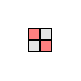
\begin{tikzpicture}[scale=0.3]
			\draw[fill=gray!20,draw=black] (0,0) rectangle (1,1);
			\draw[fill=red!50,draw=black] (0,0.5) rectangle (0.5,1);
			\draw[fill=red!50,draw=black] (0.5,0) rectangle (1,0.5);
\end{tikzpicture}}}$ $\cdot$ of low-rank times HODLR.
\end{enumerate}
\end{multicols}
\only<6-9>{\[
\begin{split}
c_{H \cdot H}(n) = & 2 \left( c_{H \cdot H}(\nicefrac{n}{2}) + \alert<7>{c_{\text{LR} \cdot \text{LR}}(\nicefrac{n}{2})} + \alert<8>{c_{H \cdot \text{LR} }(\nicefrac{n}{2})} + \alert<8>{c_{\text{LR} \cdot H}(\nicefrac{n}{2})} \right. \\ & \left. + \alert<8>{c_{H + \text{LR}}(\nicefrac{n}{2})} + c_{\text{LR}+\text{LR}}(\nicefrac{n}{2}) \right)
\end{split}
\]}
\only<7>{$c_{\text{LR} \cdot \text{LR}}(n) = 4 n k^2$}\only<8>{$c_{H\cdot\text{LR}}(n) = c_{\text{LR}\cdot H} = k c_{H\mathbf{v}}(n) = k(4k+1)\log_2(n)n$}\only<9>{$c_{H+\text{LR}}(n) = c_{H + H}(n) = c_{\text{SVD}}(nk^3 + n \log(n)k^2)$}
\only<10>{
\faMoneyCheck\;Total cost $c_{H \cdot H}(n)  \in O(k^3 n \log n + k^2 n \log^2 n).$
}
\end{frame}

\begin{frame}{BLAS with HODLR format}
\emph{Approximate} solution of a linear system $A \mathbf{x} = \mathbf{b}$ with HODLR matrix $A$:
\begin{description}
	\item[$A \approx LU$]<2-> Approximate LU-factorization $A \approx LU$ in HODLR format:
\[
\vcenter{\hbox{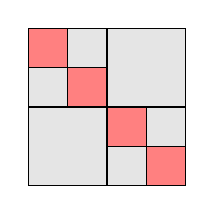
\begin{tikzpicture}
			% outerblock
			\draw[fill=gray!20,draw=black] (0,0) rectangle (1,1);
			\draw[fill=gray!20,draw=black] (1,0) rectangle (2,1);
			\draw[fill=gray!20,draw=black] (0,-1) rectangle (1,0);
			\draw[fill=gray!20,draw=black] (1,-1) rectangle (2,0);
			%inblocks (1,1)
			\draw[fill=red!50,draw=black] (0,0.5) rectangle (0.5,1);
			\draw[fill=red!50,draw=black] (0.5,0) rectangle (1,0.5);
			%inblocks (2,2)
			\draw[fill=red!50,draw=black] (1,-0.5) rectangle (1.5,0);
			\draw[fill=red!50,draw=black] (1.5,-1) rectangle (2,-0.5);
\end{tikzpicture}}} \approx 		\vcenter{\hbox{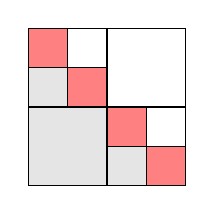
\begin{tikzpicture}
% outerblock
\draw[draw=black] (0,0) rectangle (1,1);
\draw[draw=black] (1,0) rectangle (2,1);
\draw[fill=gray!20,draw=black] (0,-1) rectangle (1,0);
\draw[draw=black] (1,-1) rectangle (2,0);
\draw[fill=gray!20,draw=black] (0,0) rectangle (0.5,0.5);
\draw[fill=gray!20,draw=black] (1,-1) rectangle (1.5,-0.5);
%inblocks (1,1)
\draw[fill=red!50,draw=black] (0,0.5) rectangle (0.5,1);
\draw[fill=red!50,draw=black] (0.5,0) rectangle (1,0.5);
%inblocks (2,2)
\draw[fill=red!50,draw=black] (1,-0.5) rectangle (1.5,0);
\draw[fill=red!50,draw=black] (1.5,-1) rectangle (2,-0.5);
\end{tikzpicture}}} \cdot 		\vcenter{\hbox{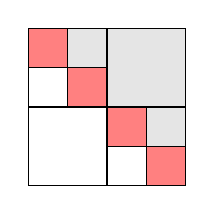
\begin{tikzpicture}
% outerblock
\draw[draw=black] (0,0) rectangle (1,1);
\draw[fill=gray!20,draw=black] (1,0) rectangle (2,1);
\draw[draw=black] (0,-1) rectangle (1,0);
\draw[draw=black] (1,-1) rectangle (2,0);
\draw[fill=gray!20,draw=black] (0.5,0.5) rectangle (1,1);
\draw[fill=gray!20,draw=black] (1.5,-0.5) rectangle (2,0);
%inblocks (1,1)
\draw[fill=red!50,draw=black] (0,0.5) rectangle (0.5,1);
\draw[fill=red!50,draw=black] (0.5,0) rectangle (1,0.5);
%inblocks (2,2)
\draw[fill=red!50,draw=black] (1,-0.5) rectangle (1.5,0);
\draw[fill=red!50,draw=black] (1.5,-1) rectangle (2,-0.5);
\end{tikzpicture}}}
\]	
	\item[Forward]<3-> substitution to solve $L\mathbf{y} = \mathbf{b}$,
	\item[Backward]<3-> substitution to solve $U \mathbf{x} = \mathbf{y}$.
\end{description}

\onslide<4>{
\begin{center}
	We need to analyze the two steps separately.
\end{center}
}

\end{frame}

\begin{frame}{BLAS with HODLR format}
	Approximate LU factorization, on level $\ell = 1$:
	\[
	A = \begin{bmatrix}
		A_{11} & A_{12} \\
		A_{21} & A_{22}
	\end{bmatrix}, \quad L = \begin{bmatrix}
		L_{11} & O \\
		L_{21} & L_{22}
	\end{bmatrix}, \quad U = \begin{bmatrix}
		U_{11} & U_{12} \\
		O & U_{22}
	\end{bmatrix}
	\]
	It is done in four steps
	\begin{enumerate}
		\item<2-> Compute LU factors $L_{11}$, $U_{11}$ of $A_{11}$,
		\item<3-> Compute $U_{12} = L_{11}^{-1} A_{12}$ by \textbf{forward substitution},
		\item<4-> Compute $L_{21} = A_{21} U_{11}^{-1}$ by \textbf{backward substitution},
		\item<5-> Compute LU factors $L_{22}$, $U_{22}$ of $A_{22} - L_{21}U_{12}$. 
	\end{enumerate}
	
	\onslide<6->{
		The analysis of the cost is \emph{analogous to the matrix-matrix multiplication case}, \textbf{but} we \alert{need to know how to do and how-much does forward/backward substitution costs}.
	}
	
\end{frame}

\begin{frame}{BLAS with HODLR format}
Forward substitution with lower triangular $L$ in HODLR format: $\mathbf{y} = L^{-1}\mathbf{b}$
\[
L = \begin{bmatrix}
	L_{11} & O \\
	L_{21} & L_{22}
\end{bmatrix}, \quad \mathbf{y} = \begin{bmatrix}
\mathbf{y}_1 \\
\mathbf{y}_2
\end{bmatrix}, \quad \mathbf{b} = \begin{bmatrix}
\mathbf{b}_1 \\
\mathbf{b}_2
\end{bmatrix}
\]
with $L_{21}$ low-rank, and $L_{11}$, $L_{22}$ HODLR.
\begin{enumerate}
	\item<2-> Solve $L_{11}\mathbf{y}_1 = \mathbf{b}_1$,
	\item<3-> Compute $\tilde{\mathbf{b}}_2 = \mathbf{b}_2 - L_{21}\mathbf{y}_1$,
	\item<4-> Solve $L_{22}\mathbf{y}_2 = \tilde{\mathbf{b}}_2$.
\end{enumerate}
\onslide<5->{Cost recursively:
\[
c_{\text{forw}} = 2 c_{\text{forw}}(\nicefrac{n}{2}) + (2k+1)n.
\]
}\onslide<6->{
On level $\ell = p$, we have the direct solution of $2^p = \nicefrac{n}{n_0}$ linear systems of size $n_0 \times n_0$.
}

\onslide<7->{\faMoneyCheck\; Total cost $c_{\text{forw}} \in O(kn\log(n))$, and \alert{analogously for backward substitution}.}

\onslide<8->{\faMoneyCheck\; Total cost $c_{\text{LU}}(n) \lesssim c_{H \cdot H}(n) \in O(k^3 n \log n + k^2 n \log^2 n)$. }
\end{frame}

\begin{frame}{BLAS with HODLR format}

\begin{columns}
\begin{column}{0.5\columnwidth}
The \href{https://github.com/numpi/hm-toolbox}{\faGithub}\,\texttt{hm-toolbox}~\parencite{MR4082285} contains all the routines.

\begin{itemize}
	\item[\faCode] They \emph{overload} the standard MATLAB operation by the same name, i.e., if you have variables in the right class you operate directly in this format.
	\item[\faSeedling] One can use different \textbf{cluster tree} $\mathcal T_p$ to get smaller ranks. They are determined by the partitioning of the index set on the leaf level and represented as the vector $\mathbf{c} = [n_{1}^{(p)},\dots,n_{2^p}^{(p)}]$, change it to change the HODLR matrix. 
\end{itemize}

\end{column}
\begin{column}{0.5\columnwidth}
\centering
\begin{tabular}{c|c}
	\toprule
	Operation&HODLR complexity \\
	\hline
	\mintinline{matlab}{A*v}&$\mathcal O(kn\log n)$\\
	\mintinline{matlab}{A\v}&$\mathcal O(k^2n\log^2 n)$\\
	\mintinline{matlab}{A+B}&$\mathcal O(k^2n\log n)$\\
	\mintinline{matlab}{A*B}&$\mathcal O(k^2n\log^2 n)$\\
	\mintinline{matlab}{A\B}&$\mathcal O(k^2n\log^2 n)$\\
	\mintinline{matlab}{inv(A)}&$\mathcal O(k^2n\log^2 n)$\\
	\mintinline{matlab}{A.*B}\footnotemark[2]&$\mathcal O(k^4n\log n)$\\
	\mintinline{matlab}{ lu(A), chol(A)}&$\mathcal O(k^2n\log^2 n)$\\
	\mintinline{matlab}{qr(A)}&$\mathcal O(k^2n\log^2 n)$\\
	compression&$\mathcal O(k^2n\log(n))$\\
	\bottomrule
\end{tabular}

\end{column}
\end{columns}
\footnotetext[2]{The complexity of the Hadamard product is dominated by the recompression stage due to the $k^2$ HODLR rank of $A\circ B$. Without recompression the cost is $\mathcal O(k^2n\log n)$.}
\end{frame}

\begin{frame}[fragile]{HODLR solver for the 1D case}

We can modify our first example to get a solution for the 1D problem in the new format.\vspace{-1em}

\begin{columns}
\begin{column}{0.6\columnwidth}
\definecolor{bg}{rgb}{0.95,0.95,0.95}
\begin{minted}[bgcolor=bg,fontsize=\small,breaklines]{matlab}
%% Discretization
N = 2^7; hN = 1/(N-1);  x = 0:hN:1; dt = hN;
alpha = 1.5; % Coefficients
dplus=@(x)gamma(3-alpha).*x.^alpha;
dminus=@(x)gamma(3-alpha).*(1-x).^alpha;
w = @(x) 5*x.*(1-x);
tol = 1e-9; % HODLR building
tic;
G = glhodlrmatrix(N,alpha,tol);
Dplus = hodlr('diagonal',dplus(x));
Dminus = hodlr('diagonal',dminus(x));
I = hodlr('eye', N);
nu = hN^alpha/dt;
A = nu*I -(Dplus*G + Dminus*G');
buildtime = toc;
\end{minted}
\end{column}
\begin{column}{0.4\columnwidth}
\definecolor{bg}{rgb}{0.95,0.95,0.95}
\begin{minted}[bgcolor=bg,fontsize=\small,breaklines]{matlab}
%% Solving
[L,U] = lu(A);
flu = @() lu(A);
timelu = timeit(flu,2);
w = w(x).';
solvetime = 0;
for i=1:N
 tic;
 w = U\(L\(nu*w));
 solvetime = solvetime + toc;
end
solvetime = solvetime/N;
\end{minted}
\vspace{-1em}\begin{itemize}
	\item[\faClock]<2-> Let us try looking at the timings.
\end{itemize}
\end{column}
\end{columns}

\end{frame}

\begin{frame}[fragile]{HODLR solver for the 1D case}

We take $\alpha = 1.5$, and $\varepsilon = 10^{-9}$
\begin{columns}
\begin{column}{0.5\columnwidth}
\begin{center}
	\begin{tabular}{cccc}
		\toprule
		$N$ & Build (s) & LU (s) & Avg. Solve (s) \\
		\midrule
		$2^{7}$ & 8.96e-03 & 1.44e-04 & 2.93e-04 \\
		$2^{8}$ & 1.35e-02 & 4.63e-04 & 3.33e-04 \\
		$2^{9}$ & 3.14e-02 & 2.05e-03 & 5.41e-04 \\
		$2^{10}$ & 7.28e-02 & 6.21e-03 & 9.35e-04 \\
		$2^{11}$ & 1.59e-01 & 1.63e-02 & 1.75e-03 \\
		$2^{12}$ & 3.85e-01 & 4.33e-02 & 3.68e-03 \\
		$2^{13}$ & 8.81e-01 & 1.27e-01 & 7.99e-03 \\
		$2^{14}$ & 2.19e+00 & 3.73e-01 & 1.55e-02 \\
		\bottomrule
	\end{tabular}
\end{center}
\end{column}
\begin{column}{0.5\columnwidth}
\centering
\only<1>{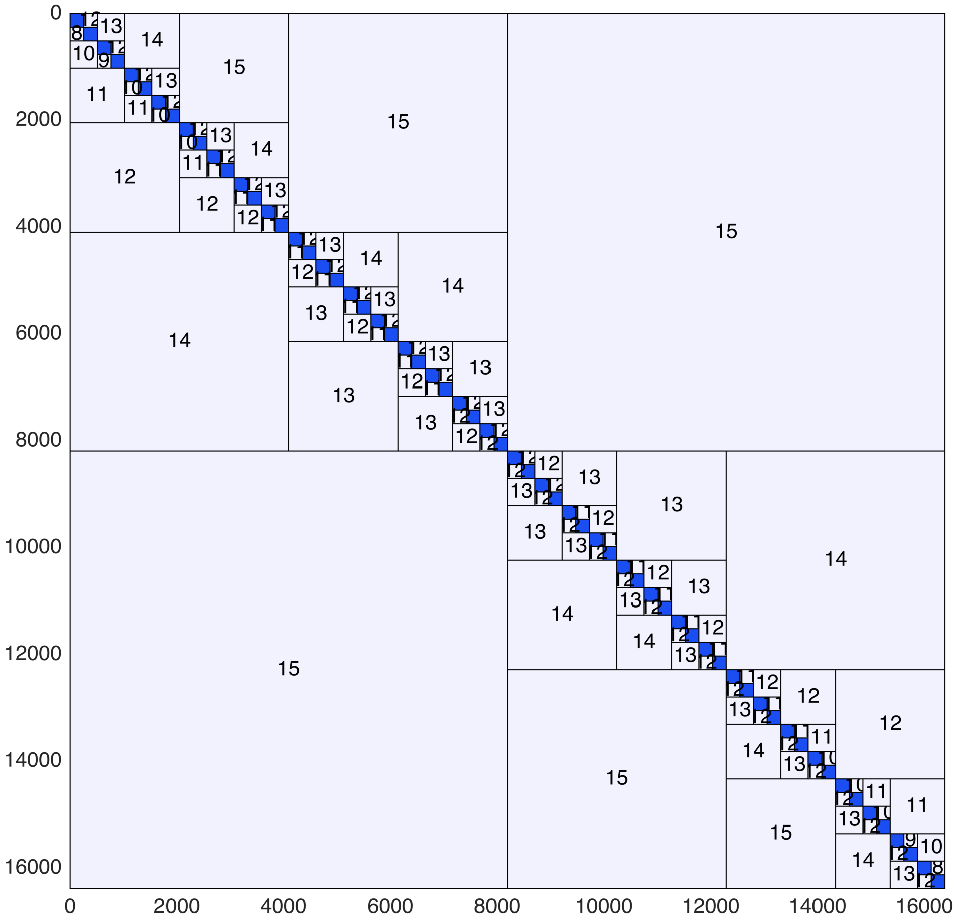
\includegraphics[width=0.8\columnwidth]{An.pdf}}%
\only<2>{% This file was created by matlab2tikz.
%
%The latest updates can be retrieved from
%  http://www.mathworks.com/matlabcentral/fileexchange/22022-matlab2tikz-matlab2tikz
%where you can also make suggestions and rate matlab2tikz.
%
\definecolor{mycolor1}{rgb}{0.00000,0.44700,0.74100}%
\definecolor{mycolor2}{rgb}{0.85000,0.32500,0.09800}%
\definecolor{mycolor3}{rgb}{0.92900,0.69400,0.12500}%
%
\begin{tikzpicture}

\begin{axis}[%
width=0.75\columnwidth,
height=1.5in,
at={(0in,0in)},
scale only axis,
xmode=log,
xmin=100,
xmax=16384,
xminorticks=true,
xlabel style={font=\color{white!15!black}},
xlabel={$N$},
ymode=log,
ymin=0.0001,
ymax=10,
yminorticks=true,
ylabel style={font=\color{white!15!black}},
ylabel={Time (second)},
axis background/.style={fill=white},
legend style={at={(3.5in,0.5in)}, legend cell align=left, align=left, draw=none, fill=none}
]
\addplot [color=mycolor1, line width=2.0pt, mark=square, mark options={solid, mycolor1}]
  table[row sep=crcr]{%
128	0.008958\\
256	0.013521\\
512	0.031421\\
1024	0.072773\\
2048	0.158879\\
4096	0.38483\\
8192	0.880753\\
16384	2.190584\\
};
\addlegendentry{Build time (s)}

\addplot [color=mycolor2, line width=2.0pt, mark=o, mark options={solid, mycolor2}]
  table[row sep=crcr]{%
128	0.0001437415\\
256	0.0004628905\\
512	0.0020548055\\
1024	0.0062138055\\
2048	0.0162558055\\
4096	0.0433198055\\
8192	0.1265308055\\
16384	0.3733568055\\
};
\addlegendentry{LU time (s)}

\addplot [color=mycolor3, line width=2.0pt, mark=x, mark options={solid, mycolor3}]
  table[row sep=crcr]{%
128	0.000292890625\\
256	0.0003327421875\\
512	0.000541173828125\\
1024	0.000935428710937501\\
2048	0.001751888671875\\
4096	0.00367795141601563\\
8192	0.00799334423828128\\
16384	0.0155332114868165\\
};
\addlegendentry{Avg. solve time (s)}

\end{axis}
\end{tikzpicture}%}%
\only<3>{% This file was created by matlab2tikz.
%
%The latest updates can be retrieved from
%  http://www.mathworks.com/matlabcentral/fileexchange/22022-matlab2tikz-matlab2tikz
%where you can also make suggestions and rate matlab2tikz.
%
\definecolor{mycolor1}{rgb}{0.00000,0.44700,0.74100}%
\definecolor{mycolor2}{rgb}{0.85000,0.32500,0.09800}%
\definecolor{mycolor3}{rgb}{0.92900,0.69400,0.12500}%
%
\begin{tikzpicture}

\begin{axis}[%
width=0.75\columnwidth,
height=1.5in,
at={(0.772in,0.473in)},
scale only axis,
xmin=128,
xmax=16384,
xlabel style={font=\color{white!15!black}},
xlabel={$N$},
ymode=log,
ymin=1,
ymax=2597.41832038764,
yminorticks=true,
ylabel style={font=\color{white!15!black}},
ylabel={Speedup},
axis background/.style={fill=white},
legend style={at={(0.97,0.03)}, anchor=south east, legend cell align=left, align=left, draw=none, fill=none}
]
\addplot [color=mycolor1, line width=2.0pt, mark=square, mark options={solid, mycolor1}]
  table[row sep=crcr]{%
128	1\\
256	1.50937709310114\\
512	3.50759098012949\\
1024	8.12379995534718\\
2048	17.7359901763787\\
4096	42.9593659298951\\
8192	98.3202723822282\\
16384	244.539406117437\\
};
\addlegendentry{Build time}

\addplot [color=mycolor2, line width=2.0pt, mark=o, mark options={solid, mycolor2}]
  table[row sep=crcr]{%
128	1\\
256	3.22029824372224\\
512	14.2951444085389\\
1024	43.2290291947698\\
2048	113.090551441303\\
4096	301.372989011524\\
8192	880.266349662415\\
16384	2597.41832038764\\
};
\addlegendentry{LU time}

\addplot [color=mycolor3, line width=2.0pt, mark=x, mark options={solid, mycolor3}]
  table[row sep=crcr]{%
128	1\\
256	1.13606295012003\\
512	1.84769938650307\\
1024	3.19378167511336\\
2048	5.98137503334222\\
4096	12.5574228127501\\
8192	27.2912259935984\\
16384	53.0341709872634\\
};
\addlegendentry{Avg. solve time}

\end{axis}
\end{tikzpicture}%}
\end{column}
\end{columns}
\vfill

\onslide<1->{\faMemory\;Largest matrix occupies 46.25 Mb, against the 2 Gb of the dense storage and the 0.87 Mb of storing three diagonals and $2 \times (2N-1)$ for the Toeplitz storage.}

\end{frame}

\subsection{Back to Sylvester}

\begin{frame}{Back to Sylvester~\parencite{MR3867617}}

To solve the Sylvester equation with HODLR coefficients
\[
A X + X B^T = C, \qquad A \in \mathbb{R}^{n \times n}, \;\; B \in \mathbb{R}^{m \times m}, \;\; X,C \in \mathbb{R}^{n \times m},
\]
we can use the integral formulation
\[
X=\int_0^{+\infty}e^{-At}Ce^{-B^T t}\,\mathrm{d}t.
\]
\onslide<2>{We perform the \emph{change of variables}: $t=f(\theta) \triangleq L\cdot\cot\left(\frac{\theta}{2}\right)^2$, rewriting the integral as
\[
X=2L\int_0^{\pi}\frac{\sin(\theta)}{(1-\cos(\theta))^2} \ e^{-Af(\theta)}Ce^{-B^T f(\theta)}\,\mathrm{d}\theta,
\]	
with $L$ a parameter to be optimized for convergence.
}
\end{frame}

\begin{frame}{Back to Sylvester~\parencite{MR3867617}}
We now have an integral on a finite domain $\Rightarrow$ \textbf{Gauss-Legendre quadrature}
\[
X\approx\sum_{j=1}^m\omega_j\cdot e^{-Af(\theta_j)}Ce^{-B^Tf(\theta_j)},  
\]
for
$\{ \theta_j, w_j \}_{j=1}^{m}$ are the Legendre points and weights, and $\omega_j=2 L w_j \cdot \frac{\sin(\theta_j)}{ (1 - \cos(\theta_j))^2
}$.
\onslide<2->{

\faQuestionCircle\;The \alert{\textbf{dominant cost}} is now computing $e^{-Af(\theta_j)}$ and $e^{-B^Tf(\theta_j)}$, how do we do it?
}
\begin{itemize}
	\item[\faCode]<3-> A \textbf{good idea} could be using \emph{rational approximation} to $\exp(t)$
	\item[\faDoorOpen]<4-> $(d, d)$-Padé with \emph{scaling and squaring} $e^{A} = (e^{2^{-k} A})^{2^k}$ and $k = \lceil \log_2 \|A\|_2 \rceil$.
	\item[\faDoorOpen]<5-> Rational Chebyshev function~\parencite{MR2421464}:
	 \[
	e^{x} \approx \frac{r_1}{x - s_1} + \ldots + \frac{r_d}{x - s_d}. 
	\]
	requiring $d$ inversions and additions that is uniformly accurate for every positive value of $t$, and thus is better in the case in which $\|A\|_2$ is large.
\end{itemize}
\end{frame}

\begin{frame}{Back to Sylvester~\parencite{MR3867617}}
\begin{columns}
\begin{column}{0.5\columnwidth}\small
\begin{algorithm}[H]
\KwIn{lyap\_integral}{$A,B,C,m$}\;
\tcc{Solves $AX + XB^T = C$ with $m$ integration points}
$L \gets 100$ \tcc*{Should be tuned for accuracy!}
$[w,\theta] \gets \operatorname{GaussLegendrePts}{m}$ \tcc*{Integration points and weights on $[0,\pi]$}
$X \gets 0_{n \times n}$\;
\For{$i = 1, \ldots, m$}{
$f \gets L \cdot \cot(\frac{\theta_i}{2})^2$\;
$X \gets X + w_i \frac{\sin(\theta_i)}{(1 - \cos \theta_i)^2} \cdot\;
\operatorname{expm}{(-f \cdot A)} \cdot C \cdot \operatorname{expm}{(-f \cdot B^T)}$\;
}
$X \gets 2L \cdot X$\;
\end{algorithm}
\end{column}
\begin{column}{0.5\columnwidth}
\begin{exampleblock}<2->{Mixed structures}
If the right-hand side $C$ is low-rank, and the structure in
the matrices $A$ and $B$ is HODLR, thus permitting to perform
fast matrix vector multiplications and system solutions; then we can apply the \emph{extended Krylov subspace
	method} we had already seen.
\end{exampleblock}
\only<3->{Build \only<4->{$\mathbb{EK}_s(A, U)$, $\mathbb{EK}_s(B^T, V)$, project on }
\only<3>{\begin{align*}
	\mathbb{EK}_s(A, U) &= \mathrm{span}\{ U, A^{-1}U, AU, \ldots\} \\
	\mathbb{EK}_s(B^T, V) &= \mathrm{span}\{ V, B^{-T}V, B^T V, \ldots\},
\end{align*}}\only<4->{
$\tilde A_s = U_s^* A U_s$, $\tilde B_s = V_s^* B V_s$,
$\tilde U = U_s^* U$, and $\tilde V = V_s^* V$.
}\only<5->{ Solve $\tilde A_s X_s + X_s \tilde B_s = \tilde U \tilde V^T$ with \textbf{dense arithmetic}.} \only<6->{An approximation is $U_s X_sV_s^*$.}\only<7->{ Another viable approach in the literature is~\parencite{MR3928351}.}
}
\end{column}
\end{columns}
\end{frame}

\begin{frame}{A numerical test~\parencite{MR3995304}}
	
We use the usual square $[0, 1]^2$, and the source $f$
\[
f(x,y,t) = 100 \cdot \left(\sin(10 \pi x) \cos(\pi y) +
\sin(10 t) \sin(\pi x) \cdot y (1 - y) \right).
\]
for both \textbf{constant coefficient} $d^+ = d^- = 1$, and variable coefficients
 \begin{align*}
 	\begin{split}
 		d_{1}^{+}(x) &= \Gamma(1.2) (1 + x)^{\alpha_1}, \qquad
 		d_{1}^{-}(x) = \Gamma(1.2) (2 - x)^{\alpha_1},  \\
 		d_{2}^{+}(y) &= \Gamma(1.2) (1 + y)^{\alpha_2}, \qquad
 		d_{2}^{-}(y) = \Gamma(1.2) (2 - y)^{\alpha_2}.
 	\end{split}
 \end{align*}
The fractional orders are $\alpha_1 = 1.3, \alpha_2 = 1.7$, and $\alpha_1 = 1.7, \alpha_2 = 1.9$.
Methods are
\begin{itemize}
	\item[\faHammer] Sylvester by Extended-Krylov with stopping $\epsilon = 10^{-6}$ (HODLR),
	\begin{itemize}
		\item[\faWrench] HODLR arithmetic is set to work with a truncation of $10^{-8}$.
	\end{itemize}
	\item[\faHammer] Sylvester by Extended-Krylov with stopping $\epsilon = 10^{-6}$ \parencite{MR3498143},
	\begin{itemize}
		\item[\faWrench] Inner solve with: GMRES with tolerance $10^{-7}$ and \emph{structured preconditioners},
	\end{itemize}
\end{itemize}
\end{frame}

\begin{frame}[fragile]{A numerical test~\parencite{MR3995304}}

Constant coefficient with $\alpha_1 = 1.3$ and $\alpha_2 = 1.7$.

\begin{columns}
\begin{column}{0.5\columnwidth}
\pgfplotstabletypeset[
columns={0,1,5,2,3},
every head row/.style={before row=\toprule,after row=\midrule},	% style the first row
every last row/.style={after row=\bottomrule},	% style the last row
columns/0/.style = {column name = $N$},
columns/1/.style = {column name = $t_{\mathrm{HODLR}}$},
columns/2/.style = {column name = $\mathrm{rank}_{\epsilon}$},
columns/5/.style = {column name = $t_{\mathrm{BSS}}$},
columns/3/.style={column name=$\text{qsrank}_\epsilon$}
]{fd-times_13.dat}
\end{column}
\begin{column}{0.5\columnwidth}
\begin{tikzpicture}
	\begin{loglogaxis}[width = 0.95\columnwidth, legend pos = north west,
		xlabel = $N$, ylabel = Time (s)]
		\addplot table[x index = 0, y index = 1] {fd-times_13.dat};
		\addplot table[x index = 0, y index = 5] {fd-times_13.dat};
		\legend{HODLR, BSS}
	\end{loglogaxis}
\end{tikzpicture}
\end{column}
\end{columns}
\vfill

\faCode\; \mintinline{bash}{FD_Example.m} from \href{https://github.com/numpi/fme}{\faGithub\;github.com/numpi/fme}

\end{frame}

\begin{frame}[fragile]{A numerical test~\parencite{MR3995304}}
Constant coefficient with $\alpha_1 = 1.7$ and $\alpha_2 = 1.9$.

\begin{columns}
	\begin{column}{0.5\columnwidth}
		\pgfplotstabletypeset[
		columns={0,1,5,2,3},
		every head row/.style={before row=\toprule,after row=\midrule},	% style the first row
		every last row/.style={after row=\bottomrule},	% style the last row
		columns/0/.style = {column name = $N$},
		columns/1/.style = {column name = $t_{\mathrm{HODLR}}$},
		columns/2/.style = {column name = $\mathrm{rank}_{\epsilon}$},
		columns/5/.style = {column name = $t_{\mathrm{BSS}}$},
		columns/3/.style={column name=$\text{qsrank}_\epsilon$}
		]{fd-times_24.dat}
	\end{column}
	\begin{column}{0.5\columnwidth}
		\begin{tikzpicture}
			\begin{loglogaxis}[width = 0.95\columnwidth, legend pos = north west,
				xlabel = $N$, ylabel = Time (s)]
        		\addplot table[x index = 0, y index = 1] {fd-times_24.dat};
				\addplot table[x index = 0, y index = 5] {fd-times_24.dat};
				\legend{HODLR, BSS}
			\end{loglogaxis}
		\end{tikzpicture}
	\end{column}
\end{columns}
\vfill

\faCode\; \mintinline{bash}{FD_Example.m} from \href{https://github.com/numpi/fme}{\faGithub\;github.com/numpi/fme}
\end{frame}

\begin{frame}[fragile]{A numerical test~\parencite{MR3995304}}
Non-constant coefficient case with $\alpha_1 = 1.3$ and $\alpha_2 = 1.7$.

\begin{columns}
	\begin{column}{0.5\columnwidth}
		\pgfplotstabletypeset[
		columns={0,1,5,2,3},
		every head row/.style={before row=\toprule,after row=\midrule},	% style the first row
		every last row/.style={after row=\bottomrule},	% style the last row
		columns/0/.style = {column name = $N$},
		columns/1/.style = {column name = $t_{\mathrm{HODLR}}$},
		columns/2/.style = {column name = $\mathrm{rank}_{\epsilon}$},
		columns/5/.style = {column name = $t_{\mathrm{BSS}}$},
		columns/3/.style={column name=$\text{qsrank}_\epsilon$}
		]{fd-times-vc_13.dat}
	\end{column}
	\begin{column}{0.5\columnwidth}
		\begin{tikzpicture}
			\begin{loglogaxis}[width = 0.95\columnwidth, legend pos = north west,
				xlabel = $N$, ylabel = Time (s)]
    			\addplot table[x index = 0, y index = 1] {fd-times-vc_13.dat};
				\addplot table[x index = 0, y index = 5] {fd-times-vc_13.dat};
				\legend{HODLR, BSS}
			\end{loglogaxis}
		\end{tikzpicture}
	\end{column}
\end{columns}
\vfill

\faCode\; \mintinline{bash}{FD_Example_vc.m} from \href{https://github.com/numpi/fme}{\faGithub\;github.com/numpi/fme}

\end{frame}

\begin{frame}[fragile]{A numerical test~\parencite{MR3995304}}
	Non-constant coefficient case with $\alpha_1 = 1.7$ and $\alpha_2 = 1.9$.
	
	\begin{columns}
		\begin{column}{0.5\columnwidth}
			\pgfplotstabletypeset[
			columns={0,1,5,2,3},
			every head row/.style={before row=\toprule,after row=\midrule},	% style the first row
			every last row/.style={after row=\bottomrule},	% style the last row
			columns/0/.style = {column name = $N$},
			columns/1/.style = {column name = $t_{\mathrm{HODLR}}$},
			columns/2/.style = {column name = $\mathrm{rank}_{\epsilon}$},
			columns/5/.style = {column name = $t_{\mathrm{BSS}}$},
			columns/3/.style={column name=$\text{qsrank}_\epsilon$}
			]{fd-times-vc_24.dat}
		\end{column}
		\begin{column}{0.5\columnwidth}
			\begin{tikzpicture}
				\begin{loglogaxis}[width = 0.95\columnwidth, legend pos = north west,
					xlabel = $N$, ylabel = Time (s)]
					\addplot table[x index = 0, y index = 1] {fd-times-vc_24.dat};
					\addplot table[x index = 0, y index = 5] {fd-times-vc_24.dat};
					\legend{HODLR, BSS}
				\end{loglogaxis}
			\end{tikzpicture}
		\end{column}
	\end{columns}
\vfill

\faCode\; \mintinline{bash}{FD_Example_vc.m} from \href{https://github.com/numpi/fme}{\faGithub\;github.com/numpi/fme}
\end{frame}

\begin{frame}{\Large The tale of the matrix equation: the moral of the story.}

\begin{itemize}
	\item[\faClock]<1-> There is an advantage with respect to using Toeplitz-based BLAS like operations,
	\item[\faForward]<2-> In~\parencite{MR3995304} they are solving the case
	\[\hspace{-3.2em}
	\left( \frac{1}{2} I_{N_x} - \Delta t \tilde{G}_{N_x} \right) \tilde{W}^{(m+1)} + \tilde{W}^{(m+1)} \left( \frac{1}{2} I_{N_y} - \Delta t \tilde{G}_{N_y} \right)^T = \tilde{W}^{(m)} + \Delta t F^{(m+1)}, \;\, m=0,\ldots,M-1.
	\]
	here the spectrum is \emph{fictitiously independent from the discretization}, i.e., all matrix-equation solvers perform a number of iteration independent from the system size: the cost is reduced to the extended Krylov subspace cost! \alert{\textbf{But}} we still have time-stepping to do.
	\item[\faQuestionCircle]<3-> The case in which the matrix equation solver has a number of iterations dependent on the problem size is not yet resolved:
	\begin{center}
		\faSmile\,Low-rank \emph{but} \alert{\textbf{\faSadCry\,no preconditioner}} -- VS -- \alert{\textbf{\faSadCry\,Full memory}} \emph{but} \faSmile\,preconditioners
	\end{center}
	\item[\faExclamation]<4-> Still looking for a way to solve \textbf{everything} \emph{all-at-once} \underline{compactly}. 
\end{itemize}

\end{frame}


\section{Conclusion and summary}

\begin{frame}{Conclusion and summary}
	\definecolor{success}{HTML}{4a934a}
	\definecolor{todo}{HTML}{0099cc}
	
	\begin{itemize}
		\item[\textcolor{success}{\faCheckCircle}] We have seen how to work with matrices in HODLR format,
		\item[\textcolor{success}{\faCheckCircle}] We have discussed a couple of strategy to solve Sylvester equations with HODLR coefficients,
		\item[\textcolor{success}{\faCheckCircle}] We have applied all the machinery to solve a time step of a 2D equation FDE.
	\end{itemize}
	\vfill

	Next up
	\begin{itemize}
		\item[\textcolor{todo}{\faClipboardList}] Back to \emph{all-at-once} solution with respect to both space and time,
		\item[\textcolor{todo}{\faClipboardList}] Linear multistep formulas in boundary value form,
		\item[\textcolor{todo}{\faClipboardList}] Structured preconditioner for LMFs,
		\item[\textcolor{todo}{\faClipboardList}] Tensor-Train reformulation of the problem.
	\end{itemize}
	
\end{frame}

	
	\section*{Bibliography}
	{\unnumbered
		\begin{frame}[allowframebreaks,noframenumbering]{Bibliography}
			\small
			\printbibliography
			
		\end{frame}
	}
\end{document}